% =====================================================================
% IEEE Transactions on Vehicular Technology -- INTERNAL DRAFT v0.1
% Merges the two WCNC 2027 submissions [P1] natanzi2027wcncA and
% [P2] natanzi2027wcncB and adds the planned journal extensions.
%
% COLOUR CODE (remove before submission):
%   black  = text rewritten from the conference versions; numbers are the
%            macros of numbers_p1.tex / numbers_p2.tex (WCNC held-out
%            seeds) and MUST be regenerated for the journal configuration
%   orange = new method or analysis proposed for the journal version;
%            design not yet implemented or validated
%   red    = TBD: new results, figures, or facts still to be produced or
%            verified. NO number in red may be invented.
% =====================================================================
\documentclass[journal]{IEEEtran}
\usepackage{cite}
\usepackage{amsmath,amssymb,amsfonts}
\usepackage{algorithm}
\usepackage{algpseudocode}
\usepackage{graphicx}
\usepackage{booktabs}
\usepackage{multirow}
\usepackage{siunitx}
\usepackage{xcolor}
\usepackage{tikz}
\usetikzlibrary{arrows.meta,patterns,positioning,fit,calc}
\usepackage[hidelinks]{hyperref}

\definecolor{propcol}{RGB}{204,102,0}
\newcommand{\tbd}[1]{\textcolor{red}{[TBD: #1]}}
\newcommand{\newres}{\textcolor{red}{[TBD]}}
\newenvironment{proposed}{\color{propcol}}{}

% Generated by scripts/make_paper.py from results/. Do not edit.
\newcommand{\numEventsPerMin}{8.5}
\newcommand{\numBusShare}{41--42\%}
\newcommand{\numPedShare}{58--59\%}
\newcommand{\numSameCellLoss}{26--33}
\newcommand{\numOtherCellBus}{58--61\%}
\newcommand{\numOtherCellPed}{29--30\%}
\newcommand{\numOnsetBus}{0.47}
\newcommand{\numOnsetPed}{$\le$0.001}
\newcommand{\numBusPd}{0.94}
\newcommand{\numPedPd}{0.48}
\newcommand{\numFA}{3.8}
\newcommand{\numLeadBus}{83--90\%}
\newcommand{\numLeadPed}{53--65\%}
\newcommand{\numMapBus}{0.83 to 0.91}
\newcommand{\numMapPed}{0.28 to 0.45}
\newcommand{\numMapCross}{2.1 to 0.4}
\newcommand{\numGhostGain}{0.83 to 0.88}
\newcommand{\numRefMargin}{35.9}
\newcommand{\numSNRreq}{9.3}
\newcommand{\numOverhead}{2.3\%}
\newcommand{\numAthreeTen}{3.58}
\newcommand{\numAthreeRef}{0.21}
\newcommand{\numAthreeWideRef}{0.16}
\newcommand{\numGenieTen}{3.64}
\newcommand{\numOracleTen}{3.04}
\newcommand{\numOracleRef}{0.03}
\newcommand{\numAfiveTen}{3.51}
\newcommand{\numAfiveRef}{0.09}
\newcommand{\numCostOracleTen}{3.13}
\newcommand{\numCostOracleRef}{0.03}
\newcommand{\numGeniePlanTen}{3.17}
\newcommand{\numGeniePlanRef}{0.04}
\newcommand{\numSensePlanTen}{10.34}
\newcommand{\numSensePlanRef}{0.19}
\newcommand{\numTrueLossRef}{0.05}
\newcommand{\numTrueLossFrom}{15}
\newcommand{\numPairedMaxP}{0.084}
\newcommand{\numRelRedTen}{11\%}
\newcommand{\numTrueLossSigFrom}{20}
\newcommand{\numBEPosSigMax}{0.125}
\newcommand{\numBEUESigMax}{0.075}
\newcommand{\numTrueLossSigMaxP}{0.049}
\newcommand{\numCalPedAcq}{1.2}
\newcommand{\numCalPedOut}{0.9}
\newcommand{\numCalPosErr}{0.53--1.84}
\newcommand{\numGridCost}{1.9\%}
\newcommand{\numOnsetPedFast}{62\%}
\newcommand{\numErrMissTen}{+2.71}
\newcommand{\numErrFalseTen}{+0.70}
\newcommand{\numErrNoiseTen}{+1.30}
\newcommand{\numErrAllTen}{+4.92}
\newcommand{\numErrMissRef}{+0.108$^\dagger$}
\newcommand{\numErrFalseRef}{+0.006$^\dagger$}
\newcommand{\numErrNoiseRef}{+0.049}
\newcommand{\numErrAllRef}{+0.099}
\newcommand{\numDensLowTen}{1.76}
\newcommand{\numDensHighTen}{5.26}
\newcommand{\numRelRedRefLow}{88\%}
\newcommand{\numRelRedRefHigh}{59\%}
\newcommand{\numAbsRedTen}{0.38}
\newcommand{\numRelRedRef}{62\%}
\newcommand{\numAbsRedRef}{0.057}
\newcommand{\numValueRange}{73--88\%}
\newcommand{\numValuePedRange}{48--65\%}
\newcommand{\numValueBusRange}{10--29\%}
\newcommand{\numValuePedTen}{53\%}
\newcommand{\numValueBusTen}{29\%}
\newcommand{\numPlanHorizon}{0.5}
\newcommand{\numSensePlanHO}{25.3}
\newcommand{\numSensePlanPP}{0.56}
\newcommand{\numAfiveHO}{6.6}
\newcommand{\numGeniePlanShareRange}{62--79\%}
\newcommand{\numGeniePlanShareTen}{73\%}
\newcommand{\numErrPerfTen}{+0.33}
\newcommand{\numErrPerfRef}{-0.042}
\newcommand{\numErrSizeTen}{+0.89}
\newcommand{\numErrSizeRef}{-0.018$^\dagger$}
\newcommand{\numErrAllUETen}{+6.91}
\newcommand{\numErrAllUERef}{+0.101}
\newcommand{\numErrRealTen}{+6.83}
\newcommand{\numErrRealRef}{+0.099}
\newcommand{\numMissPerFrameTen}{+0.87}
\newcommand{\numBEPosRange}{0.12--0.17}
\newcommand{\numBEUERange}{0.08--0.13}
\newcommand{\numBEPosRef}{0.64}
\newcommand{\numBEUERef}{0.19}
\newcommand{\numUAK}{8}
\newcommand{\numUAThetaTen}{0.3}
\newcommand{\numUAThetaRef}{0.1}
\newcommand{\numUAPlanIntervene}{6.6\%}
\newcommand{\numUAPlanTen}{+0.37}
\newcommand{\numUAPlanRef}{+0.008}
\newcommand{\numAfiveOHTen}{+0.37}
\newcommand{\numAfiveOHRef}{+0.002}
\newcommand{\numUAvsOHRef}{+0.006$^\dagger$}
\newcommand{\numBEVelMin}{$>$1}
\newcommand{\numBEPosSigRange}{0--0.125}
\newcommand{\numBEUESigRange}{0--0.075}
\newcommand{\numUAAlpha}{1}
\newcommand{\numUATheta}{0.3/0.1}
\newcommand{\numUAKTen}{8}
\newcommand{\numUAKRef}{8}
\newcommand{\numUAAlphaTen}{1}
\newcommand{\numUAAlphaRef}{1}
\newcommand{\numUAvsOHTen}{+0.00$^\dagger$}
\newcommand{\numRobustTen}{+3.01}
\newcommand{\numRobustRef}{+0.025}
\newcommand{\numHybridTen}{6.04}
\newcommand{\numGenieRef}{0.24}
\newcommand{\numHybridRef}{0.36}
\newcommand{\numXappTen}{6.71}
\newcommand{\numGenieMatch}{79\%}
\newcommand{\numAthreeMatch}{43\%}
\newcommand{\numGeniePreBus}{65\%}
\newcommand{\numAthreePreBus}{22\%}
\newcommand{\numForesightRange}{2--11\%}
\newcommand{\numForesightRef}{10\%}
\newcommand{\numForesightMaxAbs}{0.31}
\newcommand{\numTauZeroLow}{35--41\%}
\newcommand{\numTauZeroHigh}{61--95\%}
\newcommand{\numTauZeroRef}{97\%}

% Generated by scripts/p2_make_paper.py from results/P2 (heldout2 seeds). Do not edit.
\newcommand{\pAfiveFifteen}{1.88}
\newcommand{\pAfiveRef}{0.058}
\newcommand{\pAniso}{3.0}
\newcommand{\pArray}{\ensuremath{8\times8}}
\newcommand{\pBinM}{5}
\newcommand{\pBlockedDb}{10}
\newcommand{\pBootN}{10{,}000}
\newcommand{\pBreakEven}{8--13}
\newcommand{\pBreakEvenMedDist}{9--15}
\newcommand{\pBreakEvenRms}{11--18}
\newcommand{\pBusCountHigh}{2}
\newcommand{\pBusCountLow}{1}
\newcommand{\pBusLaneKmHigh}{12.5}
\newcommand{\pBusLaneKmLow}{6.25}
\newcommand{\pBusLaneMinHigh}{6}
\newcommand{\pBusLaneMinLow}{3}
\newcommand{\pBwA}{100}
\newcommand{\pBwB}{200}
\newcommand{\pBwC}{400}
\newcommand{\pCarCountHigh}{12}
\newcommand{\pCarCountLow}{4}
\newcommand{\pCarLaneKmHigh}{75}
\newcommand{\pCarLaneKmLow}{25}
\newcommand{\pCarLaneMinHigh}{45}
\newcommand{\pCarLaneMinLow}{15}
\newcommand{\pCarSpeed}{8--12}
\newcommand{\pCarrier}{28}
\newcommand{\pCi}{95}
\newcommand{\pClockBias}{50}
\newcommand{\pCloseEstCapFifteen}{+0.525}
\newcommand{\pCloseEstCapRef}{+0.051}
\newcommand{\pCloseEstCapThirty}{+0.118}
\newcommand{\pCloseEstCapTwenty}{+0.434}
\newcommand{\pCloseEstCapTwentyFive}{+0.251}
\newcommand{\pCloseEstFifteen}{+0.652}
\newcommand{\pCloseEstIdealFifteen}{+0.584}
\newcommand{\pCloseEstIdealRef}{+0.054}
\newcommand{\pCloseEstIdealThirty}{+0.121}
\newcommand{\pCloseEstIdealTwenty}{+0.483}
\newcommand{\pCloseEstIdealTwentyFive}{+0.295}
\newcommand{\pCloseEstRef}{+0.052}
\newcommand{\pCloseEstThirty}{+0.118}
\newcommand{\pCloseEstTwenty}{+0.507}
\newcommand{\pCloseEstTwentyFive}{+0.284}
\newcommand{\pCloseFullLosFifteen}{+0.162}
\newcommand{\pCloseFullLosRef}{+0.097}
\newcommand{\pCloseFullLosThirty}{+0.151}
\newcommand{\pCloseFullLosTwenty}{+0.301}
\newcommand{\pCloseFullLosTwentyFive}{+0.175}
\newcommand{\pCloseFullMapFifteen}{-0.099}
\newcommand{\pCloseFullMapRef}{-0.005$^\dagger$}
\newcommand{\pCloseFullMapThirty}{+0.021$^\dagger$}
\newcommand{\pCloseFullMapTwenty}{-0.049$^\dagger$}
\newcommand{\pCloseFullMapTwentyFive}{-0.044}
\newcommand{\pCloseOracleFifteen}{+0.461}
\newcommand{\pCloseOracleRef}{+0.048}
\newcommand{\pCloseOracleThirty}{+0.115}
\newcommand{\pCloseOracleTwenty}{+0.443}
\newcommand{\pCloseOracleTwentyFive}{+0.260}
\newcommand{\pClosePebLosFifteen}{+0.165}
\newcommand{\pClosePebLosRef}{+0.087}
\newcommand{\pClosePebLosThirty}{+0.179}
\newcommand{\pClosePebLosTwenty}{+0.286}
\newcommand{\pClosePebLosTwentyFive}{+0.187}
\newcommand{\pClosePebMapFifteen}{-0.095}
\newcommand{\pClosePebMapRef}{-0.009$^\dagger$}
\newcommand{\pClosePebMapThirty}{+0.010$^\dagger$}
\newcommand{\pClosePebMapTwenty}{-0.038$^\dagger$}
\newcommand{\pClosePebMapTwentyFive}{-0.041}
\newcommand{\pClosePerfFifteen}{-0.108}
\newcommand{\pClosePerfRef}{-0.025}
\newcommand{\pClosePerfThirty}{-0.007$^\dagger$}
\newcommand{\pClosePerfTwenty}{-0.066$^\dagger$}
\newcommand{\pClosePerfTwentyFive}{-0.061}
\newcommand{\pCloseWhiteFifteen}{+1.402}
\newcommand{\pCloseWhiteRef}{+0.117}
\newcommand{\pCloseWhiteThirty}{+0.290}
\newcommand{\pCloseWhiteTwenty}{+0.824}
\newcommand{\pCloseWhiteTwentyFive}{+0.476}
\newcommand{\pCommStep}{10}
\newcommand{\pCurbY}{4.25}
\newcommand{\pDecLosFourHundredAll}{74\%}
\newcommand{\pDecLosFourHundredBlk}{47\%}
\newcommand{\pDecLosFourHundredLos}{84\%}
\newcommand{\pDecLosHundredAll}{72\%}
\newcommand{\pDecLosHundredBlk}{46\%}
\newcommand{\pDecLosHundredLos}{81\%}
\newcommand{\pDecLosTwoHundredAll}{73\%}
\newcommand{\pDecLosTwoHundredBlk}{47\%}
\newcommand{\pDecLosTwoHundredLos}{82\%}
\newcommand{\pDecMapFourHundredAll}{99\%}
\newcommand{\pDecMapFourHundredBlk}{95\%}
\newcommand{\pDecMapFourHundredLos}{100\%}
\newcommand{\pDecMapHundredAll}{97\%}
\newcommand{\pDecMapHundredBlk}{90\%}
\newcommand{\pDecMapHundredLos}{100\%}
\newcommand{\pDecMapTwoHundredAll}{98\%}
\newcommand{\pDecMapTwoHundredBlk}{93\%}
\newcommand{\pDecMapTwoHundredLos}{100\%}
\newcommand{\pDecThr}{10}
\newcommand{\pDerivAgree}{38\%}
\newcommand{\pDerivAgreeValues}{77\%}
\newcommand{\pDerivDisFloat}{86\%}
\newcommand{\pDerivDisNearZero}{14\%}
\newcommand{\pDerivDisOther}{0\%}
\newcommand{\pDerivDisPathChange}{0\%}
\newcommand{\pDerivFdBestStep}{\ensuremath{10^{-4}}}
\newcommand{\pDerivFdMaxRel}{\ensuremath{3.2\times 10^{-6}}}
\newcommand{\pDerivFdNumUe}{1000}
\newcommand{\pDevAMed}{12.8}
\newcommand{\pDevAPninety}{1.87}
\newcommand{\pDevARmse}{6.3}
\newcommand{\pDevBMed}{12.3}
\newcommand{\pDevBPninety}{3.52}
\newcommand{\pDevBRmse}{12.7}
\newcommand{\pEpoch}{0.1}
\newcommand{\pEstBlkAoa}{29}
\newcommand{\pEstBlkFourHundred}{27}
\newcommand{\pEstBlkHundred}{44}
\newcommand{\pEstBlkIdealHw}{25}
\newcommand{\pEstBlkKept}{11}
\newcommand{\pEstBlkSyncEpoch}{27}
\newcommand{\pEstBlkToa}{21}
\newcommand{\pEstBlkTwoHundred}{37}
\newcommand{\pEstBlkWorstHw}{35}
\newcommand{\pEstDecAoa}{44\%}
\newcommand{\pEstDecFourHundred}{45\%}
\newcommand{\pEstDecHundred}{29\%}
\newcommand{\pEstDecIdealHw}{51\%}
\newcommand{\pEstDecKept}{52\%}
\newcommand{\pEstDecSyncEpoch}{45\%}
\newcommand{\pEstDecToa}{46\%}
\newcommand{\pEstDecTwoHundred}{34\%}
\newcommand{\pEstDecWorstHw}{34\%}
\newcommand{\pEstLosAoa}{10}
\newcommand{\pEstLosFourHundred}{10}
\newcommand{\pEstLosHundred}{20}
\newcommand{\pEstLosIdealHw}{7}
\newcommand{\pEstLosKept}{9}
\newcommand{\pEstLosSyncEpoch}{10}
\newcommand{\pEstLosToa}{10}
\newcommand{\pEstLosTwoHundred}{18}
\newcommand{\pEstLosWorstHw}{17}
\newcommand{\pEstMedAoa}{13}
\newcommand{\pEstMedFourHundred}{12}
\newcommand{\pEstMedHundred}{24}
\newcommand{\pEstMedIdealHw}{10}
\newcommand{\pEstMedKept}{9}
\newcommand{\pEstMedSyncEpoch}{12}
\newcommand{\pEstMedToa}{12}
\newcommand{\pEstMedTwoHundred}{21}
\newcommand{\pEstMedWorstHw}{20}
\newcommand{\pEstPninetyAoa}{2.14}
\newcommand{\pEstPninetyFourHundred}{2.10}
\newcommand{\pEstPninetyHundred}{4.98}
\newcommand{\pEstPninetyIdealHw}{1.50}
\newcommand{\pEstPninetyKept}{1.45}
\newcommand{\pEstPninetySyncEpoch}{2.28}
\newcommand{\pEstPninetyToa}{1.14}
\newcommand{\pEstPninetyTwoHundred}{5.59}
\newcommand{\pEstPninetyWorstHw}{5.19}
\newcommand{\pEstRmseFourHundred}{6.2}
\newcommand{\pEstRmseHundred}{6.8}
\newcommand{\pEstRmseIdealHw}{4.8}
\newcommand{\pEstToPebAoa}{2}
\newcommand{\pEstToPebFourHundred}{2}
\newcommand{\pEstToPebHundred}{4}
\newcommand{\pEstToPebIdealHw}{33}
\newcommand{\pEstToPebKept}{2}
\newcommand{\pEstToPebSyncEpoch}{2}
\newcommand{\pEstToPebToa}{2}
\newcommand{\pEstToPebTwoHundred}{3}
\newcommand{\pEstToPebWorstHw}{1}
\newcommand{\pFacadeYNorth}{9.57}
\newcommand{\pFacadeYSouth}{\ensuremath{-8.61}}
\newcommand{\pFdStep}{1}
\newcommand{\pFimJobErr}{\ensuremath{2.9\times 10^{-6}}}
\newcommand{\pFimToyErr}{\ensuremath{6.6\times 10^{-10}}}
\newcommand{\pGridSize}{144}
\newcommand{\pHeavySpeed}{6--10}
\newcommand{\pHwLosCalFive}{58\%}
\newcommand{\pHwLosIdeal}{92\%}
\newcommand{\pHwLosSyncThree}{92\%}
\newcommand{\pHwLosWorst}{44\%}
\newcommand{\pHwMapCalFive}{99\%}
\newcommand{\pHwMapIdeal}{99\%}
\newcommand{\pHwMapSyncThree}{99\%}
\newcommand{\pHwMapWorst}{98\%}
\newcommand{\pLaneWidth}{3.5}
\newcommand{\pLaneYEast}{\ensuremath{-2.5}}
\newcommand{\pLaneYWest}{2.5}
\newcommand{\pLimLosBase}{4.8}
\newcommand{\pLimLosBw}{0.97}
\newcommand{\pLimLosCal}{0.07}
\newcommand{\pLimLosSnr}{0.94}
\newcommand{\pLimLosSync}{0.72}
\newcommand{\pLimMapBase}{0.5}
\newcommand{\pLimMapBw}{0.71}
\newcommand{\pLimMapCal}{0.42}
\newcommand{\pLimMapSnr}{0.32}
\newcommand{\pLimMapSync}{0.45}
\newcommand{\pLitHigh}{0.8}
\newcommand{\pLitLow}{0.6}
\newcommand{\pLoopDelay}{20}
\newcommand{\pMapToLosBlk}{0.09}
\newcommand{\pMapToLosP}{0.002}
\newcommand{\pMarginFifteen}{15}
\newcommand{\pMarginTwenty}{20}
\newcommand{\pMaxDepth}{2}
\newcommand{\pMaxPaths}{8}
\newcommand{\pMirrorAMed}{12}
\newcommand{\pMirrorAPninety}{1.90}
\newcommand{\pMirrorARmse}{6.36}
\newcommand{\pMirrorAboveP}{95\%}
\newcommand{\pMirrorOfTopTen}{48\%}
\newcommand{\pMirrorOracleMed}{11}
\newcommand{\pMirrorOraclePninety}{1.19}
\newcommand{\pMirrorOracleRmse}{1.83}
\newcommand{\pMirrorShareEpochs}{5\%}
\newcommand{\pNoiseFig}{7}
\newcommand{\pNscA}{792}
\newcommand{\pNscB}{1584}
\newcommand{\pNscC}{3168}
\newcommand{\pNumEl}{64}
\newcommand{\pNumRuns}{40}
\newcommand{\pNumSeeds}{10}
\newcommand{\pNumerology}{3}
\newcommand{\pOnsetDuringMed}{87}
\newcommand{\pOnsetDuringPninety}{3.26}
\newcommand{\pOnsetDuringShQuarter}{72\%}
\newcommand{\pOnsetDuringShTen}{88\%}
\newcommand{\pOnsetElseMed}{10}
\newcommand{\pOnsetElsePninety}{1.59}
\newcommand{\pOnsetElseShQuarter}{29\%}
\newcommand{\pOnsetElseShTen}{49\%}
\newcommand{\pOnsetNumEvents}{752}
\newcommand{\pOnsetPreHalfMed}{11}
\newcommand{\pOnsetPreHalfPninety}{4.49}
\newcommand{\pOnsetPreHalfShQuarter}{29\%}
\newcommand{\pOnsetPreHalfShTen}{53\%}
\newcommand{\pOnsetPreOneMed}{12}
\newcommand{\pOnsetPreOnePninety}{4.24}
\newcommand{\pOnsetPreOneShQuarter}{30\%}
\newcommand{\pOnsetPreOneShTen}{54\%}
\newcommand{\pOruOffset}{40}
\newcommand{\pOruOneFacX}{\ensuremath{-40}}
\newcommand{\pOruOneFacY}{\ensuremath{-7}}
\newcommand{\pOruOneFacZ}{5}
\newcommand{\pOruOneLampX}{\ensuremath{-28}}
\newcommand{\pOruOneLampY}{\ensuremath{-7}}
\newcommand{\pOruOneLampZ}{5}
\newcommand{\pOruZeroFacX}{0}
\newcommand{\pOruZeroFacY}{9.2}
\newcommand{\pOruZeroFacZ}{8}
\newcommand{\pOruZeroLampX}{12}
\newcommand{\pOruZeroLampY}{6.5}
\newcommand{\pOruZeroLampZ}{5}
\newcommand{\pOverhead}{2.3\%}
\newcommand{\pPartOneRatio}{2.0}
\newcommand{\pPebLosFourHundredAll}{4.7}
\newcommand{\pPebLosFourHundredBlk}{11.6}
\newcommand{\pPebLosFourHundredLos}{4.1}
\newcommand{\pPebLosHundredAll}{4.9}
\newcommand{\pPebLosHundredBlk}{12.2}
\newcommand{\pPebLosHundredLos}{4.4}
\newcommand{\pPebLosTwoHundredAll}{4.8}
\newcommand{\pPebLosTwoHundredBlk}{11.8}
\newcommand{\pPebLosTwoHundredLos}{4.3}
\newcommand{\pPebMapFourHundredAll}{0.3}
\newcommand{\pPebMapFourHundredBlk}{1.2}
\newcommand{\pPebMapFourHundredLos}{0.3}
\newcommand{\pPebMapHundredAll}{0.7}
\newcommand{\pPebMapHundredBlk}{2.4}
\newcommand{\pPebMapHundredLos}{0.6}
\newcommand{\pPebMapTwoHundredAll}{0.5}
\newcommand{\pPebMapTwoHundredBlk}{1.7}
\newcommand{\pPebMapTwoHundredLos}{0.4}
\newcommand{\pPedCrossingHigh}{4}
\newcommand{\pPedCrossingLow}{2}
\newcommand{\pPedSidewalkKmHigh}{75}
\newcommand{\pPedSidewalkKmLow}{37.5}
\newcommand{\pPedSpeed}{1.0--1.5}
\newcommand{\pPedWalkersHigh}{12}
\newcommand{\pPedWalkersLow}{6}
\newcommand{\pPhiList}{0, 2 and 5}
\newcommand{\pPhiMain}{2}
\newcommand{\pPhiWorst}{5}
\newcommand{\pPlanH}{0.5--3}
\newcommand{\pRatioLosA}{1.2}
\newcommand{\pRatioLosB}{2.8}
\newcommand{\pRatioMapA}{3.7}
\newcommand{\pRatioMapB}{4.6}
\newcommand{\pRatioPLosA}{0.004}
\newcommand{\pRatioPLosB}{0.002}
\newcommand{\pRatioPMapA}{0.002}
\newcommand{\pRatioPMapB}{0.002}
\newcommand{\pRatioPtwo}{2}
\newcommand{\pRatioThr}{5}
\newcommand{\pRefMargin}{35.9}
\newcommand{\pRelMapFifteen}{\ensuremath{-}5.2\%}
\newcommand{\pRelMapRef}{\ensuremath{-}8.2\%$^\dagger$}
\newcommand{\pRelPerfFifteen}{\ensuremath{-}5.7\%}
\newcommand{\pRelPerfRef}{\ensuremath{-}43.1\%}
\newcommand{\pRunDuration}{60}
\newcommand{\pSNRreq}{9.3}
\newcommand{\pSameCellLoss}{26--33}
\newcommand{\pScs}{120}
\newcommand{\pSeedsDev}{1001--1010}
\newcommand{\pSeedsHeld}{3001--3010}
\newcommand{\pSeedsTune}{101--105}
\newcommand{\pSensRange}{40}
\newcommand{\pSidewalkNorthHi}{9.57}
\newcommand{\pSidewalkNorthLo}{4.25}
\newcommand{\pSidewalkSouthHi}{\ensuremath{-4.25}}
\newcommand{\pSidewalkSouthLo}{\ensuremath{-8.61}}
\newcommand{\pSidewalkYNorth}{6.5}
\newcommand{\pSidewalkYSouth}{\ensuremath{-7}}
\newcommand{\pStreetLen}{125}
\newcommand{\pStreetPeriod}{80}
\newcommand{\pStreetWidth}{18.2}
\newcommand{\pStreetWidthSetback}{18.9}
\newcommand{\pSyncList}{0, 0.3, 1 and 3}
\newcommand{\pSyncMain}{1}
\newcommand{\pSyncWorst}{3}
\newcommand{\pTauHO}{20}
\newcommand{\pTruckCountHigh}{2}
\newcommand{\pTruckCountLow}{1}
\newcommand{\pTruckLaneKmHigh}{12.5}
\newcommand{\pTruckLaneKmLow}{6.25}
\newcommand{\pTruckLaneMinHigh}{6}
\newcommand{\pTruckLaneMinLow}{3}
\newcommand{\pTxPower}{23}
\newcommand{\pUeHeight}{1.5}
\newcommand{\pUeSpeed}{1.0--1.2}
\newcommand{\pUeXMax}{40}
\newcommand{\pUeXMin}{\ensuremath{-40}}
\newcommand{\pUeY}{\ensuremath{-7}}
\newcommand{\pValBiasBlk}{1.8--3.0}
\newcommand{\pValBiasLos}{0.01--14.96}
\newcommand{\pValBiasMseFour}{98--100\%}
\newcommand{\pValBiasMseFourOther}{38\%}
\newcommand{\pValBiasToRmseFour}{0.62--1.00}
\newcommand{\pValBiasToRmseHundred}{0.72--1.00}
\newcommand{\pValCenToPebFour}{0.077--13}
\newcommand{\pValCenToPebHundred}{0.05--77}
\newcommand{\pValIdentity}{5e-13}
\newcommand{\pValNumDraws}{500}
\newcommand{\pValNumGeom}{6}
\newcommand{\pValRmseToPeb}{1--359}
\newcommand{\pValSpreadToPeb}{0.9--13.3}
\newcommand{\pVehCountHigh}{16}
\newcommand{\pVehCountLow}{6}
\newcommand{\pVehLaneKmHigh}{100}
\newcommand{\pVehLaneKmLow}{37.5}
\newcommand{\pVehLaneMinHigh}{57}
\newcommand{\pVehLaneMinLow}{21}
\newcommand{\pVehSpeed}{6--12}
\newcommand{\pVerdictFour}{mixed}
\newcommand{\pVerdictOneLos}{not supported}
\newcommand{\pVerdictOneMap}{not supported}
\newcommand{\pVerdictThree}{supported}
\newcommand{\pVerdictThreeKept}{supported}
\newcommand{\pVerdictTwo}{supported}
\newcommand{\pVerdictTwoKept}{not supported}


\newcommand{\placeholder}[3]{%
  \fbox{\parbox[c][#2][c]{#1}{\centering\small
  \textcolor{red}{Placeholder (new result): #3}}}}

\begin{document}

\title{ISAC-Assisted Blockage-Aware Proactive Handover in mmWave Open RAN:
Localization Requirements, Map-Aided Multipath Positioning, and
End-to-End Performance}

\author{Seyed~Bagher~Hashemi~Natanzi,~\IEEEmembership{Student Member,~IEEE,}
and~Bo~Tang,~\IEEEmembership{Member,~IEEE}% <- VERIFY membership grades
\thanks{Manuscript received \tbd{date}. This material is based upon work
supported in part by NSF under Awards CNS-2120442 and IIS-2325863, and
NTIA under Award No.\ 51-60-IF007.}%
\thanks{The authors are with the Department of Electrical and Computer
Engineering, Worcester Polytechnic Institute, Worcester, MA 01609 USA
(e-mail: snatanzi@wpi.edu; btang1@wpi.edu). Corresponding author:
S.~B.~Hashemi Natanzi.}%
\thanks{Parts of this work were submitted to IEEE WCNC 2027
\cite{natanzi2027wcncA,natanzi2027wcncB}. \tbd{update with the
acceptance status and DOI once known.}}}

\markboth{IEEE Transactions on Vehicular Technology,~Vol.~XX, No.~X, Month~2027}%
{Hashemi Natanzi and Tang: ISAC-Assisted Blockage-Aware Proactive Handover in mmWave Open RAN}

\maketitle

\begin{abstract}
Millimeter-wave (mmWave) links collapse within milliseconds when a
pedestrian or a large vehicle crosses the line of sight (LoS), and
reactive handover reacts only once the outage has begun. Integrated
sensing and communication (ISAC) could let the radio access network see
blockers in advance and move users to another cell before the link
breaks. This paper examines the complete chain that such a scheme
requires, from sensing the blockers through localizing the user to
deciding the handover, within an Open RAN (O-RAN) architecture. We first
define the value of foresight through a cost-aware oracle and show, in a
ray-traced \SI{28}{GHz} street canyon, that perfect foresight closes
\numValueRange{} of the outage gap between service-aware reactive
handover (3GPP A5) and an ideal oracle, but that harvesting it requires
the user to be localized to about one decimeter per axis. We then derive
position error bounds for uplink sounding-reference-signal positioning
that include synchronization and array calibration errors, and show that
the bound is calibration-limited and degrades sharply during blockage
unless reflected paths with known geometry from a digital twin are
exploited. \textcolor{propcol}{To close the gap between this map-aided
bound and practical estimators, we propose a blockage-aware map-aided
multipath tracker in which the blocker tracks of the ISAC radar predict
the visibility of every LoS and reflected path and thus steer data
association, and an uncertainty-aware handover planner that consumes the
resulting position covariance.} \tbd{One to two sentences with the main
quantitative results of the new tracker, the end-to-end comparison with
A3, A5, conditional handover, and sensing-aided baselines, and the E2
control-loop latency measured on an OpenAirInterface/FlexRIC testbed.}
\end{abstract}

\begin{IEEEkeywords}
Integrated sensing and communication (ISAC), millimeter wave, blockage,
proactive handover, positioning, position error bound, multipath-assisted
localization, digital twin, Open RAN.
\end{IEEEkeywords}

% ---------------------------------------------------------------------
\section{Introduction}
% ---------------------------------------------------------------------
\IEEEPARstart{T}{he} large bandwidths available in the mmWave bands are
a cornerstone of the capacity of 5G-Advanced and 6G networks, in
particular for vehicular and dense urban use cases. The same short
wavelength that enables compact high-gain arrays, however, makes mmWave
links highly sensitive to obstruction. When a pedestrian, a bus, or a
truck crosses the LoS between a radio unit and a user equipment (UE),
the received power drops by tens of decibels within milliseconds and
may remain low for up to several seconds
\cite{rappaport2013mmwave,maccartney2017blockage}. Standardized mobility
procedures are reactive: beam failure recovery and handover are
triggered by degraded and filtered measurements, typically after a
time-to-trigger, so the user experiences at least part of every outage
\cite{3gpp38331,3gpp38300}. For services with tight reliability or
latency requirements, such as cooperative driving or extended reality,
these interruptions dominate the perceived quality.

Avoiding an outage rather than recovering from it requires knowing the
blocker before it arrives. Prior work has predicted blockage from
cameras, dedicated radars, or acoustic sensors and has used these
predictions for proactive handoff or beam management
\cite{charan2021vision,demirhan2022radarblockage,alquraan2023radar,hanahara2024acoustic}.
ISAC offers an alternative that needs no auxiliary sensor: the radio
unit observes its surroundings with its own orthogonal
frequency-division multiplexing (OFDM) waveform
\cite{liu2022isac,sturm2011ofdm}. 3GPP has studied ISAC use cases and
introduced sensing-target channel models \cite{3gpp22837,3gpp38901}, and
O-RAN lets third-party applications (xApps) in the near-real-time RAN
intelligent controller (near-RT RIC) act on such information through the
E2 interface \cite{polese2023oran,bonati2021intelligence}. Sensing-assisted
handover has accordingly attracted growing attention
\cite{li2025lookbefore,alquraan2023radar}.

Whether sensing-assisted handover pays off, however, depends on
quantities that existing studies rarely separate. The first is the
\emph{value} of foresight: how much a network with perfect knowledge of
the future channel could gain over the best reactive policy. The second
is the \emph{realizable} share of that value under realistic sensing,
positioning, and control-loop delays. Most studies report the gain of a
specific predictor over link-failure recovery or over untuned triggers,
so neither quantity is known, and it remains unclear which accuracy a
network needs. A third aspect is easily overlooked: predicting whether a
body will cross the line between a radio unit and the user requires
knowing where the user is. The prediction is therefore bounded by the
network's localization of the user, and this localization is itself
degraded precisely when a blocker obstructs the LoS.

In two companion conference papers, we studied these questions
separately. In \cite{natanzi2027wcncA}, we defined the value of foresight
and showed that it can only be harvested if the user and nearby blockers
are localized to about a decimeter. In \cite{natanzi2027wcncB}, we
derived position error bounds for uplink positioning by the serving
radio units and found that a practical estimator falls well short of the
map-aided bound, especially around blockage events. This paper unifies
both studies into a single sensing--positioning--handover framework and,
\textcolor{propcol}{as its main new contribution, closes the loop between
them: the blocker tracks produced by ISAC are used not only to predict
blockage of the communication link but also to predict which propagation
paths of the uplink positioning signal are visible, which makes the
association of reflected paths with the map robust exactly when the LoS
is lost.}

The contributions of this paper are as follows.
\begin{itemize}
\item \emph{Value of foresight and requirements.} We formulate
cost-aware cell selection with knowledge of the future signal-to-noise
ratio (SNR) as a sequential decision problem whose exact solution by
dynamic programming bounds every proactive policy, define the value of
foresight relative to tuned service-aware reactive handover, and derive
the user and blocker localization accuracy that a blockage-aware planner
requires \cite{natanzi2027wcncA}.
\item \emph{Positioning bounds under blockage.} We derive single-epoch
equivalent Fisher information for uplink sounding reference signal (SRS)
positioning by O-RAN radio units (O-RUs) with synchronization and
calibration errors as Bayesian priors, for LoS-only and map-aided
information and for two models of a blocked LoS \cite{natanzi2027wcncB}.
\textcolor{propcol}{We extend the hardware model to a physical array
with gain, phase, and element-position errors and a back plane.}
\item \textcolor{propcol}{\emph{Blockage-aware map-aided multipath
tracker.} We propose a tracker that predicts the visibility of the LoS
and of every virtual anchor from the ISAC blocker tracks, uses it in a
probabilistic data association of the extracted multipath components
with the digital-twin map, and estimates residual map offsets jointly
with the UE state.}
\item \textcolor{propcol}{\emph{Uncertainty-aware planning and an O-RAN
control loop.} We formulate a risk-aware handover planner that uses the
full position and blocker covariance, and we measure the E2 control-loop
latency on an OpenAirInterface (OAI) and FlexRIC testbed
\cite{nikaein2014oai,schmidt2021flexric} instead of assuming it.}
\item \emph{Evaluation.} Using a spatially consistent ray-traced
simulation in which every moving body is both a 3GPP radar target and a
blocker of communication paths, we evaluate the chain on held-out
scenarios against A3, A5, \textcolor{propcol}{conditional handover (CHO),
a sensing-triggered baseline in the spirit of \cite{li2025lookbefore},
and a learned blockage predictor in the spirit of
\cite{alquraan2023radar}}, and release all code.\footnote{%
\url{https://github.com/CLIS-WPI/sense2connect}}
\end{itemize}

Relative to \cite{natanzi2027wcncA,natanzi2027wcncB}, Section~V-C,
Sections~VI-B to VI-D, and Sections~\ref{sec:tracker} to \ref{sec:e2}
are new, the physical array model of Section~III-D and the planners of
Section~VI-C extend the conference versions, and all other sections
have been rewritten and condensed. \tbd{Final mapping to be checked
against the summary-of-differences document.}

The remainder of this paper is organized as follows. Section~II reviews
related work. Section~III presents the system model. Section~IV
formulates the handover problem and the value of foresight, and
Section~V derives the position error bounds. Section~VI describes the
proposed framework, Section~VII reports the evaluation, Section~VIII
discusses limitations, and Section~IX concludes the paper.

% ---------------------------------------------------------------------
\section{Related Work}
% ---------------------------------------------------------------------
\begin{table*}[t]
\centering
\caption{Comparison With Representative Related Work
\textcolor{red}{(entries for \cite{xu2025isacbeam,cui2025multiview,hanahara2024acoustic,li2025lookbefore}
to be verified against the full texts)}}
\label{tab:related}
\setlength{\tabcolsep}{3pt}
\begin{tabular}{@{}lllcccc@{}}
\toprule
Work & Sensing & UE localization & Dynamic blockers & Multi-cell HO & Control loop & Bounds / requirements\\
\midrule
Charan \emph{et al.} \cite{charan2021vision} & camera & -- & yes & yes & -- & --\\
Demirhan \& Alkhateeb \cite{demirhan2022radarblockage} & FMCW radar & -- & yes (real data) & -- & -- & --\\
RaDaR \cite{alquraan2023radar} & FMCW radar + FL & -- & yes & yes & -- & --\\
Look Before Switch \cite{li2025lookbefore} & ISAC (gNB) & UE kinematics & -- & yes & NR frame & --\\
Hanahara \emph{et al.} \cite{hanahara2024acoustic} & acoustic AoA & -- & yes & -- & -- & --\\
Xu \emph{et al.} \cite{xu2025isacbeam} & ISAC (multi-RSU) & UE tracking & -- & beam/RSU & -- & --\\
Cui \emph{et al.} \cite{cui2025multiview} & multi-BS ISAC & -- & yes & task alloc. & -- & --\\
Kim \emph{et al.} \cite{kim2022pmbm} & -- & multipath SLAM & -- & -- & -- & --\\
Li \emph{et al.} \cite{li2024bpslam} & -- & BP-based MP-SLAM & -- & -- & -- & --\\
Dong \emph{et al.} \cite{dong2026deployable} & -- & SRS + EKF & -- & -- & -- & --\\
\midrule
This work & ISAC (O-RU) & map-aided multipath & yes (3GPP targets) & yes & O-RAN, measured & value, PEB\\
\bottomrule
\end{tabular}
\end{table*}

\subsection{mmWave Blockage}
Measurement campaigns have shown that human bodies cause deep and rapid
fading at mmWave frequencies \cite{maccartney2017blockage}, and 3GPP
models blockage either stochastically (model~A) or geometrically as a
set of knife-edge screens (model~B) \cite{3gpp38901}. System-level
studies typically treat blockers statistically, which decouples the
blocker from anything the network could observe. Our simulation instead
couples every blocker to a radar target, so that the object that
attenuates a link is the same object that the sensing system detects.

\subsection{Sensing-Aided Blockage Prediction and Handover}
Charan \emph{et al.} \cite{charan2021vision} combined camera images and
wireless data to predict blockage and trigger proactive handoff.
Demirhan and Alkhateeb \cite{demirhan2022radar,demirhan2022radarblockage}
predicted beams and future blockages from a co-located automotive radar
using the real-world DeepSense~6G data \cite{alkhateeb2023deepsense}, and
Hanahara \emph{et al.} \cite{hanahara2024acoustic} exploited acoustic
angle of arrival to aid beam-search-based blockage prediction. RaDaR
\cite{alquraan2023radar} equips each small cell with a separate
frequency-modulated continuous-wave (FMCW) radar, decides from object,
base-station, and user heights whether an object obstructs the LoS, and
predicts the time to blockage with a federated model, reporting gains
over handover after link failure. Look Before Switch
\cite{li2025lookbefore} uses the ISAC capability of the gNB to track the
vehicular user and triggers handover from its predicted position and
maneuver, substantially reducing handover interruption relative to A3.
Multi-RSU ISAC beam tracking \cite{xu2025isacbeam} and multi-view ISAC
under blockage \cite{cui2025multiview} address cooperative sensing but
not handover between cells, and digital twins have been used for
blockage-aware multi-hop routing \cite{roongpraiwan2025dt}.

Our work differs in four respects. First, we sense third-party blockers
with the communication waveform rather than the user itself or an
auxiliary radar. Second, we compare against a tuned service-aware
reactive policy and a cost-aware oracle, which separates the value of
foresight from the share that a practical system realizes. Third, we
identify the localization of the user as a binding requirement and
analyze whether the infrastructure can meet it. Fourth,
\textcolor{propcol}{we use the sensing output to make the positioning
itself robust to blockage}.

\subsection{mmWave Positioning and Multipath-Assisted Localization}
Fisher information analyses have shown that the delay and angle
resolution of mmWave arrays supports sub-decimeter localization
\cite{shahmansoori2018position,abushaban2018bounds}, building on the
equivalent Fisher information framework for wideband localization
\cite{shen2010fundamental}. Multipath components that are specular
reflections from known surfaces can be interpreted as LoS paths from
virtual anchors (VAs), so that they add position information instead of
causing interference \cite{leitinger2015evaluation,witrisal2016high}.
Multipath-based simultaneous localization and mapping (MP-SLAM) estimates
the VAs jointly with the agent, for example with Poisson multi-Bernoulli
mixture filters in vehicular mmWave networks \cite{kim2022pmbm} or with
belief propagation \cite{li2024bpslam,meyer2018message}. 3GPP specifies
uplink time- and angle-based positioning from SRS \cite{3gpp38855}, and
recent work fuses multi-base-station SRS measurements with an extended
Kalman filter (EKF) \cite{dong2026deployable} or with GNSS
\cite{campolo2024gnss}. These works do not account for dynamic blockers
observed by an independent sensor and do not evaluate positioning by its
effect on mobility decisions; both are central to this paper.

\subsection{O-RAN Control of Mobility}
O-RAN research has demonstrated data-driven RAN control through xApps
\cite{polese2023oran,bonati2021intelligence} on open platforms such as
OAI and FlexRIC \cite{nikaein2014oai,schmidt2021flexric}. Recent
frameworks forward SRS-derived measurements to xApps for localization
\cite{oran2025locframework}, and FlexRIC reports sub-millisecond one-way
latency between the RAN and an xApp \cite{oai2024innovation}. Sensing-aided
handover studies, including our conference versions, have so far modelled
the E2 loop by a fixed delay; \textcolor{propcol}{here we measure it}.
% ---------------------------------------------------------------------
\section{System Model}
% ---------------------------------------------------------------------
\begin{figure*}[t]
\centering
\begin{minipage}[b]{0.60\textwidth}
\centering
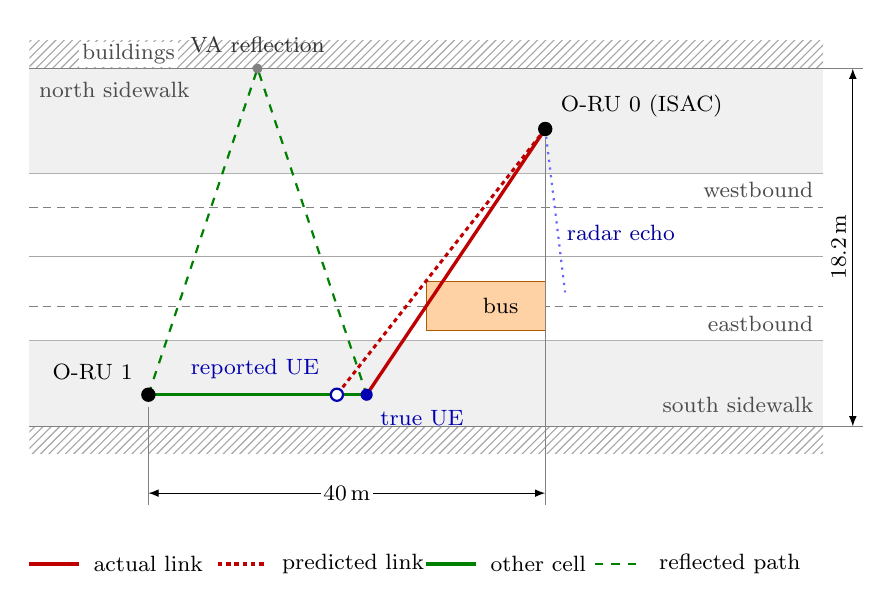
\begin{tikzpicture}[x=1.26mm,y=2.5mm,font=\footnotesize]
  \fill[pattern=north east lines,pattern color=gray!70] (-40,9.57) rectangle (40,11.0);
  \fill[pattern=north east lines,pattern color=gray!70] (-40,-8.61) rectangle (40,-10.0);
  \draw[gray] (-40,9.57)--(40,9.57); \draw[gray] (-40,-8.61)--(40,-8.61);
  \node[gray!60!black,fill=white,inner sep=1pt] at (-30,10.3) {buildings};
  \fill[gray!12] (-40,4.25) rectangle (40,9.57);
  \fill[gray!12] (-40,-8.61) rectangle (40,-4.25);
  \draw[gray!60] (-40,4.25)--(40,4.25); \draw[gray!60] (-40,-4.25)--(40,-4.25);
  \draw[densely dashed,gray] (-40,2.5)--(40,2.5); \draw[densely dashed,gray] (-40,-2.5)--(40,-2.5);
  \draw[gray!70] (-40,0)--(40,0);
  \node[gray!60!black,anchor=south east] at (40,2.5) {westbound};
  \node[gray!60!black,anchor=north east] at (40,-2.5) {eastbound};
  \node[gray!60!black,anchor=north west] at (-40,9.4) {north sidewalk};
  \node[gray!60!black,anchor=south east] at (40,-8.4) {south sidewalk};
  \draw[fill=orange!35,draw=orange!70!black] (0,-3.75) rectangle (12,-1.25);
  \node at (7.5,-2.5) {bus};
  \draw[very thick,red!75!black] (12,6.5)--(-6,-7);
  \draw[red!75!black,line width=1.1pt,dash pattern=on 1.6pt off 1.4pt] (12,6.5)--(-9,-7);
  \draw[very thick,green!50!black] (-28,-7)--(-6,-7);
  \draw[thick,green!50!black,dashed] (-28,-7)--(-17,9.57)--(-6,-7);
  \draw[blue!60,dotted,thick] (12,6.5) -- (14,-1.8);
  \node[blue!60!black,anchor=west] at (13.2,1.2) {radar echo};
  \fill[blue!70!black] (-6,-7) circle (2.2pt);
  \draw[blue!70!black,thick,fill=white] (-9,-7) circle (2.2pt);
  \node[blue!70!black,anchor=north west] at (-5.6,-7.3) {true UE};
  \node[blue!70!black,anchor=south east] at (-9.8,-6.7) {reported UE};
  \fill (12,6.5) circle (2.6pt); \node[anchor=south west] at (12.6,6.6) {O-RU 0 (ISAC)};
  \fill (-28,-7) circle (2.6pt); \node[anchor=south east] at (-28.6,-6.7) {O-RU 1};
  \fill[gray] (-17,9.57) circle (1.8pt); \node[anchor=south,gray!40!black] at (-17,9.9) {VA reflection};
  \draw[{Latex[length=1.3mm]}-{Latex[length=1.3mm]}] (-28,-12)--(12,-12);
  \draw[gray] (-28,-7.6)--(-28,-12.6); \draw[gray] (12,6)--(12,-12.6);
  \node[fill=white,inner sep=1pt] at (-8,-12) {\SI{40}{m}};
  \draw[{Latex[length=1.3mm]}-{Latex[length=1.3mm]}] (43,-8.61)--(43,9.57);
  \draw[gray] (40,-8.61)--(44,-8.61); \draw[gray] (40,9.57)--(44,9.57);
  \node[rotate=90,anchor=south] at (43.3,0.5) {\SI{18.2}{m}};
  \begin{scope}[shift={(-40,-15.6)}]
    \draw[very thick,red!75!black] (0,0)--(5,0); \node[anchor=west] at (5.5,0) {actual link};
    \draw[red!75!black,line width=1.1pt,dash pattern=on 1.6pt off 1.4pt] (19,0)--(24,0); \node[anchor=west] at (24.5,0) {predicted link};
    \draw[very thick,green!50!black] (40,0)--(45,0); \node[anchor=west] at (45.5,0) {other cell};
    \draw[thick,green!50!black,dashed] (57,0)--(62,0); \node[anchor=west] at (62.5,0) {reflected path};
  \end{scope}
\end{tikzpicture}\\[0.5mm]
{\footnotesize (a) Top view (lamppost deployment)}
\end{minipage}\hfill
\begin{minipage}[b]{0.38\textwidth}
\centering
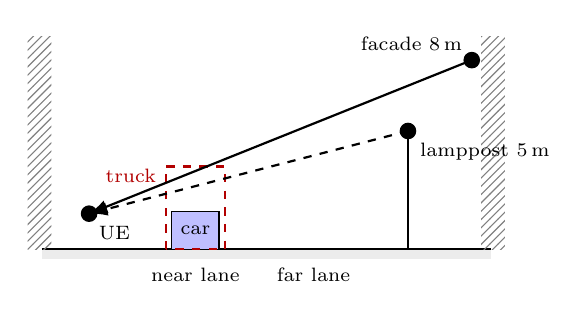
\begin{tikzpicture}[x=0.30cm,y=0.30cm,font=\scriptsize]
  \fill[gray!15] (-9,0) rectangle (10,-0.4);
  \draw[thick] (-9,0) -- (10,0);
  \fill[pattern=north east lines,pattern color=gray] (-9.6,0) rectangle (-8.6,9);
  \fill[pattern=north east lines,pattern color=gray] (9.6,0) rectangle (10.6,9);
  \node[below] at (-2.5,-0.4) {near lane};
  \node[below] at (2.5,-0.4) {far lane};
  \draw[fill=blue!25] (-3.5,0) rectangle (-1.5,1.6);
  \draw[dashed,red!70!black,thick] (-3.75,0) rectangle (-1.25,3.5);
  \node[red!70!black,left] at (-3.75,3.1) {truck};
  \node at (-2.5,0.8) {car};
  \fill (-7,1.5) circle (3pt); \node[below right] at (-7,1.4) {UE};
  \fill[black] (9.2,8) circle (3pt); \node[above left] at (9.2,8) {facade \SI{8}{m}};
  \draw[thick] (6.5,0) -- (6.5,5); \fill (6.5,5) circle (3pt);
  \node[below right] at (6.6,4.9) {lamppost \SI{5}{m}};
  \draw[thick,-{Latex}] (9.2,8) -- (-7,1.5);
  \draw[thick,dashed,-{Latex}] (6.5,5) -- (-7,1.5);
\end{tikzpicture}\\[0.5mm]
{\footnotesize (b) Street cross-section}
\end{minipage}
\caption{Scenario. (a) Two neighboring cells share a street canyon. A
position error of the reported UE turns the true serving link, which
crosses the bus, into a predicted link that passes it, so the blockage
is missed. O-RU~0 also acts as a monostatic ISAC radar; reflections from
the facades form virtual anchors (VAs). (b) Over the near lane, the LoS
passes above cars but through buses and trucks.}
\label{fig:scenario}
\end{figure*}

\subsection{Deployment}
We consider a set $\mathcal C$ of cells, each served by an O-RU with a
uniform planar array of $M$ elements, and pedestrian or vehicular UEs
with a single antenna. The reference deployment is the street canyon of
Fig.~\ref{fig:scenario}: buildings \pStreetWidth\,m apart, two
\pLaneWidth-m lanes, and sidewalks on both sides. O-RU~0 is mounted on
the north side, either on a \SI{5}{m} lamppost or on a facade at
\SI{8}{m}, and O-RU~1 on a \SI{5}{m} lamppost on the south sidewalk,
\pOruOffset\,m further along the street. Cars, buses, trucks, and
pedestrians move through a periodic section of the street; pedestrians
either walk along the sidewalks or cross the street.
\textcolor{propcol}{A second deployment (an intersection with \tbd{N}
O-RUs) is used to test generalization (Section~\ref{sec:sens}).}

\subsection{Channel and Blockage Model}
The channel from O-RU $c$ to a UE at frequency $f$ and time $t$ is
\begin{equation}
\mathbf h_c(f,t)=\sum_{\ell} 10^{-L_{c,\ell}(t)/20}\,\alpha_{c,\ell}(t)\,
\mathbf a_c(\boldsymbol\theta_{c,\ell})\,e^{-j2\pi f\tau_{c,\ell}(t)},
\label{eq:channel}
\end{equation}
where $\alpha_{c,\ell}$, $\tau_{c,\ell}$, and $\boldsymbol\theta_{c,\ell}$
are the complex gain, delay, and direction of path $\ell$ in the absence
of moving bodies, $\mathbf a_c$ is the array response, and
$L_{c,\ell}(t)$ is the loss caused by the bodies that intersect the path.
Following 3GPP blockage model~B \cite{3gpp38901}, each body $k$ acts as a
rectangular screen on every path segment it intersects, with loss
\begin{equation}
L_k=-20\log_{10}\!\bigl(1-(F_{h_1}+F_{h_2})(F_{w_1}+F_{w_2})\bigr),
\label{eq:modelB}
\end{equation}
where each knife-edge term is
$F=\pi^{-1}\arctan\bigl(\pm\tfrac{\pi}{2}\sqrt{\pi\lambda^{-1}(D_1+D_2-r)}\bigr)$
with edge distances $D_1,D_2$ and direct distance $r$; losses add in
decibels over bodies and segments. We write $\gamma_c(t)$ for the SNR of
cell $c$ and $\bar\gamma_c(t)$ for its value without moving bodies.

Model~B attenuates a blocked path but keeps its geometry, whereas the
field that actually reaches the receiver diffracts around the blocker.
For positioning, this distinction matters. We therefore distinguish a
\emph{kept} model, in which a blocked LoS retains the delay and
direction implied by the UE position, and a \emph{biased} model, in
which the blocked LoS is replaced by a detour around the dominant
blocker: with $\mathbf q$ the shortest detour point over the top or past
either side of the blocker box, the path keeps the attenuated gain but
has delay $(\|\mathbf q-\mathbf p_c\|+\|\mathbf p-\mathbf q\|)/c_0$ and
arrival direction along $\mathbf q-\mathbf p_c$, where $\mathbf p_c$ and
$\mathbf p$ are the O-RU and UE positions. \textcolor{propcol}{In
Section~\ref{sec:sens}, we compare both models with first-order diffraction traced
by Sionna~RT \tbd{verify diffraction support in the used Sionna
version}.}

\subsection{ISAC Sensing Model}
The O-RUs embed OFDM sensing symbols in their frames. With
$N_{\mathrm{sc}}$ subcarriers of spacing $\Delta f$ (bandwidth
$B=N_{\mathrm{sc}}\Delta f$) and a coherent processing interval (CPI)
of $N_s$ symbols spaced $T_s$, a monostatic radar resolves range and
radial velocity and has a maximum unambiguous velocity of
\begin{equation}
\Delta R=\frac{c_0}{2B},\qquad
\Delta v=\frac{\lambda}{2N_sT_s},\qquad
v_{\max}=\frac{\lambda}{4T_s}.
\label{eq:res}
\end{equation}
Each moving body is a 3GPP sensing target \cite{3gpp38901} with state
$\mathbf x_k(t)$ comprising position, velocity, extent, and class
(vehicles are represented by five scattering points, pedestrians by
one). The sensing O-RU operates under an ideal full-duplex assumption,
transmitting on one element and receiving on its array.
\textcolor{propcol}{A residual self-interference level is added as a
sensitivity parameter in Section~\ref{sec:sens}.}

\subsection{Uplink Positioning Signal Model}
For positioning, the UE transmits an uplink SRS that is received by all
O-RUs in $\mathcal C$. At O-RU $c$, subcarrier frequency $f_n$, and
element $m$, the received sample is
\begin{equation}
y_{c,n,m}=\sum_{\ell}\beta_{c,\ell}\,
e^{-j2\pi f_n(\tau_{c,\ell}+\delta_c+b)}\,
g_{c,m}\,s_m(\mathbf u_{c,\ell})+w_{c,n,m},
\label{eq:signal}
\end{equation}
where path $\ell$ has complex gain $\beta_{c,\ell}$ (including its
blockage loss), delay $\tau_{c,\ell}$, and arrival direction
$\mathbf u_{c,\ell}$ with steering response $s_m$; $\delta_c$ is the time
offset of O-RU $c$, $b$ the UE clock bias, and $w_{c,n,m}$ thermal noise.
In \cite{natanzi2027wcncB}, the element response was a pure calibration
phase error, $g_{c,m}=e^{j\psi_{c,m}}$ with
$\psi_{c,m}\sim\mathcal N(0,\sigma_\phi^2)$, and the steering response
was that of isotropic elements.
\begin{proposed}
Here, we use a physical array model with
$g_{c,m}=(1+\epsilon_{c,m})e^{j\psi_{c,m}}$, gain errors
$\epsilon_{c,m}\sim\mathcal N(0,\sigma_\epsilon^2)$, element-position
errors $\Delta\mathbf r_{c,m}\sim\mathcal N(\mathbf 0,\sigma_r^2\mathbf I)$
inside $s_m$, and a directional element pattern with a back plane, which
removes the front/back ambiguity of a planar array of isotropic
elements.
\end{proposed}
Synchronization errors are modelled as
$\delta_c\sim\mathcal N(0,\sigma_{\mathrm{sync}}^2)$.

\subsection{O-RAN Control Loop and Service Model}
An xApp in the near-RT RIC receives blocker tracks and UE position
estimates through E2 every $T_r$ and issues handover commands that take
effect after a loop delay $\tau_{\mathrm{E2}}$. In
\cite{natanzi2027wcncA,natanzi2027wcncB}, $\tau_{\mathrm{E2}}$ was a fixed
\SI{20}{ms}. \textcolor{propcol}{Here, $\tau_{\mathrm{E2}}$ is drawn from
the empirical distribution measured on our OAI/FlexRIC testbed
(Section~VI-D).} The UE requires a rate $R$, i.e., an SNR
$\gamma_{\mathrm{req}}$, and is in \emph{outage} whenever the SNR of its
serving cell falls below $\gamma_{\mathrm{req}}$ or the user plane is
interrupted by a handover, which lasts $\tau_{\mathrm{HO}}$.

% ---------------------------------------------------------------------
\section{Handover Problem, Value of Foresight, and Localization Requirement}
% ---------------------------------------------------------------------
\subsection{Problem Formulation}
A handover policy selects the serving cell $c_t\in\mathcal C$ at every
step $t$ of duration $\Delta t$. Its outage time over a horizon is
\begin{equation}
J(\{c_t\})=\Delta t\sum_t \mathbb 1\bigl\{\gamma_{c_t}(t)<\gamma_{\mathrm{req}}
\;\lor\; t\in\mathcal I(\{c_t\})\bigr\},
\label{eq:J}
\end{equation}
where $\mathcal I(\{c_t\})$ contains the $\tau_{\mathrm{HO}}/\Delta t$
steps after each switch, so that an interrupted step is counted once.
\emph{Reactive} policies use past measurements only. With A3, the UE
hands over when the filtered reference signal received power (RSRP) of a
neighbor exceeds that of the serving cell by an offset plus hysteresis
for a time-to-trigger; with A5, it hands over when the serving cell falls
below one threshold and the neighbor exceeds another, which makes the
policy aware of the service requirement \cite{3gpp38331}.
\textcolor{propcol}{With CHO, the target cell is prepared in advance and
the UE executes the handover autonomously once its execution condition
holds, which removes the command latency from the critical path
\cite{3gpp38331cho,3gpp38300}.}

\subsection{Oracles and the Value of Foresight}
Two bounds frame what foresight can achieve. The \emph{instantaneous
oracle} selects the better cell at every step without delay or
interruption, and thus ignores the cost of switching. The
\emph{cost-aware oracle} knows $\gamma_c(t)$ for all cells and minimizes
\eqref{eq:J} exactly. Because the cost of a step depends only on the
serving cell and the remaining interruption time, \eqref{eq:J} is
minimized by the Viterbi algorithm over the augmented state
$(c_t,\iota_t)$, where $\iota_t$ is the number of remaining interrupted
steps, with complexity $O(T|\mathcal C|^2\tau_{\mathrm{HO}}/\Delta t)$.
No policy with any predictor can do better.

We call the outage difference between the best tuned reactive policy and
the instantaneous oracle the \emph{improvable gap}, and the share of that
gap closed by the cost-aware oracle the \emph{value of foresight}. A
\emph{grid-aligned} variant restricts the oracle to the decision instants
of a practical controller and isolates the cost of that restriction.

\subsection{Localization Requirement}
A blockage-aware policy $\pi$ predicts the SNR of each cell as
\begin{equation}
\hat\gamma_c(t)=\bar\gamma_c(t)-\hat L_c(t),
\label{eq:pred}
\end{equation}
where $\bar\gamma_c$ is obtained from the digital twin and $\hat L_c$
applies \eqref{eq:modelB} to the predicted trajectories of the tracked
blockers on the line between O-RU $c$ and the reported UE position
$\hat{\mathbf p}_t=\mathbf p_t+\mathbf e_t$. Since the purpose of $\pi$ is
to outperform reactive handover, we define the localization requirement
as the set of error processes $\{\mathbf e_t\}$ for which
\begin{equation}
J\bigl(\pi;\{\hat{\mathbf p}_t\}\bigr)\le J(\mathrm{A5}).
\label{eq:req}
\end{equation}
The requirement depends on the error at the instants when the policy
acts, not only on its overall statistics, and analogous requirements
hold for the blocker state estimates $\hat{\mathbf x}_k$.

% ---------------------------------------------------------------------
\section{Position Error Bounds Under Blockage}
% ---------------------------------------------------------------------
\subsection{Equivalent Fisher Information}
Collect the channel parameters of all O-RUs at one epoch (delays, angles,
and complex gains) in $\boldsymbol\eta$, and the hardware and timing
errors in $\boldsymbol\nu=[\{\delta_c\},b,\{\psi_{c,m}\}]$. The Fisher
information matrix (FIM) of $\boldsymbol\eta$ follows from
\eqref{eq:signal} by the Slepian--Bangs formula; we evaluate it exactly
by factorizing its sums over frequency and antennas. With
$\mathbf T=\partial\boldsymbol\eta/\partial\mathbf p$, the equivalent FIM
of the position is
\begin{equation}
\mathbf J_{\mathbf p}=\mathbf T^{\mathsf T}\mathbf J_{\boldsymbol\eta}\mathbf T
-\mathbf T^{\mathsf T}\mathbf J_{\boldsymbol\eta\boldsymbol\nu}
\bigl(\mathbf J_{\boldsymbol\nu\boldsymbol\nu}+\boldsymbol\Lambda\bigr)^{-1}
\mathbf J_{\boldsymbol\nu\boldsymbol\eta}\mathbf T,
\label{eq:efim}
\end{equation}
where the nuisance parameters have been removed by Schur complements and
$\boldsymbol\Lambda$ holds the Gaussian priors of the O-RU time offsets
and element phases. The UE clock bias has no prior, so that the bound
corresponds to time-difference-of-arrival (TDoA) positioning. The
position error bound (PEB) is
$\mathrm{PEB}=\sqrt{\mathrm{tr}(\mathbf J_{\mathbf p}^{-1})}$. It bounds
the root-mean-square (RMS) error of unbiased single-epoch estimators for
a given geometry; it is not a median error, a biased estimator can have a
smaller spread, and it excludes the temporal information accumulated by
a tracking filter.

\subsection{LoS-Only and Map-Aided Information}
In the \emph{LoS-only} bound, the delays and angles of all reflected
paths are nuisance parameters, so only the LoS contributes geometric
information. In the \emph{map-aided} bound, a specular reflection on a
known surface is treated as an LoS path from the virtual anchor
$\tilde{\mathbf p}_{c,\ell}$, the image of $\mathbf p_c$ in that surface,
so that $\tau_{c,\ell}=\|\mathbf p-\tilde{\mathbf p}_{c,\ell}\|/c_0$ and
the corresponding rows of $\mathbf T$ follow analytically
\cite{leitinger2015evaluation}. In the biased model of a blocked LoS, its
delay and angles are additional nuisance parameters. We verified the
analytic derivatives against central finite differences at
\pDerivFdNumUe{} random positions (maximum relative error
\pDerivFdMaxRel), and the GPU implementation of \eqref{eq:efim} against
an independent NumPy implementation (relative deviation \pFimJobErr) and
a brute-force numerical FIM (\pFimToyErr).

\begin{proposed}
\subsection{Map-Aided Bound With an Uncertain Map}
A digital twin is never exact. Let each reflecting surface $s$ be
displaced along its normal by an unknown offset
$d_s\sim\mathcal N(0,\sigma_{\mathrm{map}}^2)$, which moves the VAs of
that surface by $2d_s\mathbf n_s$. Appending $\mathbf d=[d_s]$ to the
nuisance vector $\boldsymbol\nu$ with prior precision
$\sigma_{\mathrm{map}}^{-2}\mathbf I$ in $\boldsymbol\Lambda$ yields a
map-aided bound that degrades gracefully from the perfect-map case
($\sigma_{\mathrm{map}}\to0$) to the LoS-only case
($\sigma_{\mathrm{map}}\to\infty$). Since a surface offset is common to
all epochs and UEs, it is observable over time, which motivates
estimating it jointly with the UE state (Section~VI-B). \tbd{derive the
corresponding rows of $\mathbf T$ and verify numerically.}
\end{proposed}
% ---------------------------------------------------------------------
\section{ISAC-Assisted Handover Framework}
% ---------------------------------------------------------------------
\begin{figure*}[t]
\centering
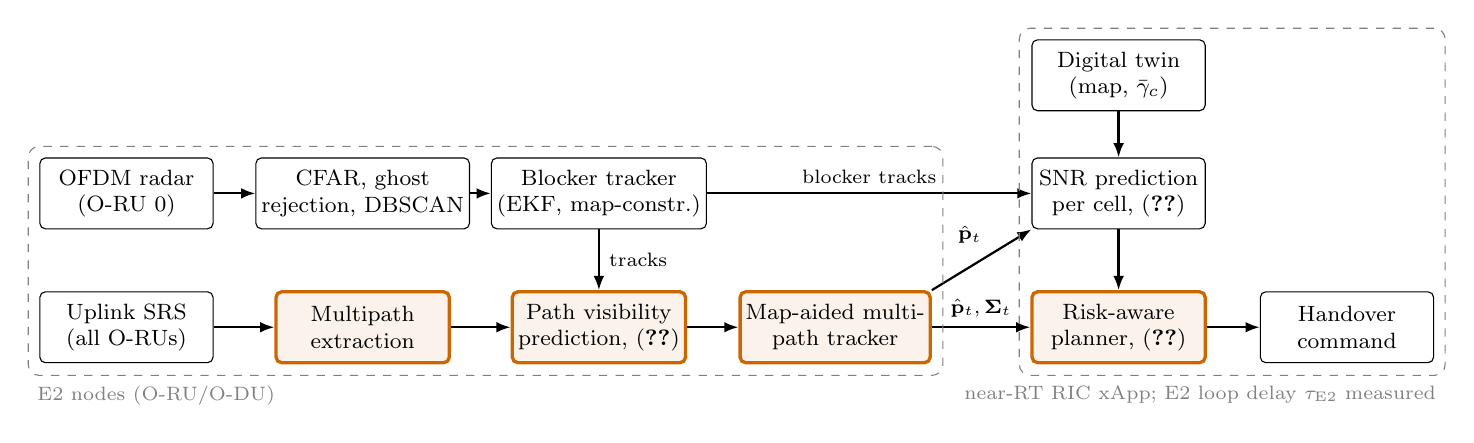
\begin{tikzpicture}[font=\footnotesize,
  blk/.style={draw,rounded corners=2pt,align=center,minimum height=9mm,minimum width=22mm,inner sep=2pt,fill=white},
  newblk/.style={blk,draw=propcol,very thick,fill=propcol!8},
  arr/.style={-{Latex[length=1.8mm]},thick},
  grp/.style={draw,dashed,gray,rounded corners=4pt,inner sep=4pt}]
  \node[blk]    (radar) at (0,0)     {OFDM radar\\(O-RU 0)};
  \node[blk]    (cfar)  at (3.0,0)   {CFAR, ghost\\rejection, DBSCAN};
  \node[blk]    (trk)   at (6.0,0)   {Blocker tracker\\(EKF, map-constr.)};
  \node[blk]    (srs)   at (0,-1.7)  {Uplink SRS\\(all O-RUs)};
  \node[newblk] (mpc)   at (3.0,-1.7) {Multipath\\extraction};
  \node[newblk] (vis)   at (6.0,-1.7) {Path visibility\\prediction, (\ref{eq:vis})};
  \node[newblk] (mat)   at (9.0,-1.7) {Map-aided multi-\\path tracker};
  \node[blk]    (dt)    at (12.6,1.5) {Digital twin\\(map, $\bar\gamma_c$)};
  \node[blk]    (pred)  at (12.6,0)   {SNR prediction\\per cell, (\ref{eq:pred})};
  \node[newblk] (plan)  at (12.6,-1.7) {Risk-aware\\planner, (\ref{eq:risk})};
  \node[blk]    (ho)    at (15.5,-1.7) {Handover\\command};
  \draw[arr] (radar)--(cfar); \draw[arr] (cfar)--(trk);
  \draw[arr] (srs)--(mpc); \draw[arr] (mpc)--(vis); \draw[arr] (vis)--(mat);
  \draw[arr] (trk)--node[right,font=\scriptsize]{tracks}(vis);
  \draw[arr] (trk)--node[above,font=\scriptsize]{blocker tracks}(pred);
  \draw[arr] (mat)--node[above,font=\scriptsize]{$\hat{\mathbf p}_t,\boldsymbol\Sigma_t$}(plan);
  \draw[arr] (mat.north east)--node[above left,font=\scriptsize,pos=0.6]{$\hat{\mathbf p}_t$}(pred.south west);
  \draw[arr] (dt)--(pred); \draw[arr] (pred)--(plan); \draw[arr] (plan)--(ho);
  \node[grp,fit=(radar)(srs)(mat)(trk)] (g1) {};
  \node[gray,anchor=north west,font=\scriptsize] at (g1.south west) {E2 nodes (O-RU/O-DU)};
  \node[grp,fit=(dt)(pred)(plan)(ho)] (g2) {};
  \node[gray,anchor=north east,font=\scriptsize] at (g2.south east) {near-RT RIC xApp; E2 loop delay $\tau_{\mathrm{E2}}$ measured};
\end{tikzpicture}
\caption{Proposed framework. Blocks with orange borders are new in this
paper. The blocker tracks of the ISAC radar feed both the SNR prediction
and the visibility prediction of the positioning paths; the digital twin
also provides the map used for ghost rejection and for the virtual
anchors.}
\label{fig:framework}
\end{figure*}

Fig.~\ref{fig:framework} summarizes the framework. The ISAC radar of the
sensing O-RU detects and tracks blockers; the O-RUs jointly localize the
UE from its uplink SRS; an xApp predicts the SNR of every cell and plans
handovers. This section describes the four components.

\subsection{Blocker Sensing and Tracking}
Per CPI, the sensing O-RU forms range--Doppler--angle maps from the
received echoes and detects targets with two-dimensional cell-averaging
constant false alarm rate (CFAR) detection. Detections that mirror real
targets on building walls known from the digital twin are rejected with
the image method, the remaining detections are clustered with DBSCAN,
and the clusters are tracked by an EKF on range, angles, and radial
velocity. Optionally, tracks are constrained to the lane center lines
(vehicles) and to the sidewalks (pedestrians, with a free motion model
for crossings). Each confirmed track $k$ provides a Gaussian state
estimate $\mathcal N(\hat{\mathbf x}_k,\mathbf P_k)$ and a class label,
which determines the extent of the screen used in \eqref{eq:modelB}.

\begin{proposed}
\subsection{Blockage-Aware Map-Aided Multipath Tracker}
The analysis of \cite{natanzi2027wcncB} showed that the information
needed for decimeter accuracy during blockage is present in the
reflected paths, but that a dominant-path estimator cannot extract it
and that a naive VA extension did not reduce the error tail. The main
difficulty is data association: when the LoS of an O-RU is blocked, the
strongest measured path is a reflection or a detour, and associating it
with the wrong source produces exactly the systematic errors observed in
\cite{natanzi2027wcncB}. The proposed tracker resolves this by
predicting, from the ISAC blocker tracks, which sources can currently be
observed.

\textit{State and sources.} The tracker estimates
$\mathbf s_t=[\mathbf p_t^{\mathsf T},\mathbf v_t^{\mathsf T},b_t,\mathbf d^{\mathsf T}]^{\mathsf T}$
with a constant-velocity model for the UE, a random walk for the clock
bias, and the surface offsets $\mathbf d$ of Section~V-C as slowly
varying parameters. For every O-RU $c$, the source set
$\mathcal S_c=\{0\}\cup\mathcal V_c$ contains the LoS and the single- and
double-bounce VAs of the map. Source $s$ predicts the measurement
$\mathbf h_{c,s}(\mathbf s_t)$ (delay, azimuth, elevation).

\textit{Multipath extraction.} Per O-RU and epoch, a sparse estimator
extracts a set $\mathcal Z_{c,t}=\{\mathbf z_j\}$ of multipath components
from \eqref{eq:signal}, \tbd{e.g., orthogonal matching pursuit on a
beam--delay grid followed by local refinement}, each with a covariance
$\mathbf R_j$ from the local Fisher information.

\textit{Visibility prediction.} Let $\mathcal G_{c,s}(\mathbf p)$ be the
polyline of source $s$ from O-RU $c$ to a UE at $\mathbf p$. Its
predicted visibility is
\begin{equation}
q_{c,s,t}=\Pr\bigl\{\mathcal G_{c,s}(\mathbf p_t)\cap\mathcal B_k(t)=\emptyset\;\;\forall k\bigr\},
\label{eq:vis}
\end{equation}
where $\mathcal B_k(t)$ is the box of blocker $k$. We evaluate
\eqref{eq:vis} with $K$ joint samples of the predicted UE state and of
the blocker states $\mathcal N(\hat{\mathbf x}_k,\mathbf P_k)$, and add
a prior blockage probability for regions that the radar does not cover.
The detection probability of source $s$ is then
$P^{\mathrm D}_{c,s,t}=q_{c,s,t}P^{\mathrm D}_{\mathrm{clr}}+(1-q_{c,s,t})P^{\mathrm D}_{\mathrm{blk}}$,
and a source that is likely blocked contributes, if detected, through a
detour model with an inflated covariance $\mathbf R^{\mathrm{blk}}$
rather than through its geometric prediction.

\textit{Data association and update.} Measurements in
$\mathcal Z_{c,t}$ are associated with sources in $\mathcal S_c$ or
declared clutter (unmodelled or diffuse paths) with a Poisson clutter
model. We compute the marginal association probabilities
$\beta_{c,j,s}$ by loopy belief propagation over the bipartite
association graph \cite{williams2014bp,meyer2018message}, which scales
linearly in the numbers of sources and measurements, and update the
state with a probabilistic data association EKF that weights the
innovation of each source by $\beta_{c,j,s}$ \cite{barshalom2009pda}.
Positions outside the walkable area of the map are rejected, and the
back plane of the physical array model removes front/back mirror
solutions.

\textit{Complexity.} Per epoch, the visibility prediction costs
$O(K\,N_{\mathrm{blk}}\sum_c|\mathcal S_c|)$ segment--box tests and the
association $O(I_{\mathrm{BP}}\sum_c|\mathcal S_c||\mathcal Z_{c,t}|)$
operations for $I_{\mathrm{BP}}$ iterations. \tbd{measured run time per
epoch on the target hardware (Table~\ref{tab:complexity}).}

\begin{algorithm}[t]
\caption{Blockage-aware map-aided multipath tracker (one epoch)}
\label{alg:tracker}
\begin{algorithmic}[1]
\Require posterior of $\mathbf s_{t-1}$; blocker tracks $\{\hat{\mathbf x}_k,\mathbf P_k\}$; map; SRS samples $\{y_{c,n,m}\}$
\State Predict $\mathbf s_{t|t-1}$ with the motion model
\State Draw $K$ joint samples of $\mathbf p_t$ and of the blocker boxes
\For{each O-RU $c$ and source $s\in\mathcal S_c$}
  \State Compute $q_{c,s,t}$ by \eqref{eq:vis} and $P^{\mathrm D}_{c,s,t}$
\EndFor
\For{each O-RU $c$}
  \State Extract multipath components $\mathcal Z_{c,t}$
  \State Gate $\mathcal Z_{c,t}$ against $\mathbf h_{c,s}(\mathbf s_{t|t-1})$
  \State Compute $\beta_{c,j,s}$ by belief propagation
\EndFor
\State PDA-EKF update of $\mathbf s_t$ with all weighted innovations
\State Enforce map constraints; output $\hat{\mathbf p}_t$ and covariance $\mathbf\Sigma_t$
\end{algorithmic}
\end{algorithm}
\end{proposed}

\subsection{SNR Prediction and Handover Planning}
At each report, the xApp predicts $\hat\gamma_c$ for all cells by
\eqref{eq:pred}. The \emph{planner} of \cite{natanzi2027wcncA} minimizes
\eqref{eq:J} on $\hat\gamma_c$ over a horizon $H$ and its decision grid
by the Viterbi algorithm and applies the first decision after the loop
delay. The \emph{genie-planner} uses the true future SNR and isolates
the effect of prediction errors. \emph{Trigger} policies, in contrast,
hand over when a LoS blockage of the serving cell is predicted and the
other cell is predicted to be clear. The \emph{uncertainty-aware
planner} of \cite{natanzi2027wcncA} keeps A5 as its default and
intervenes only when the expected outage reduction, averaged over $K$
samples of the track posteriors and of a white UE position error,
exceeds a threshold $\theta$.

\begin{proposed}
\textit{Risk-aware planner.} With the proposed tracker, the position
uncertainty is no longer a white, isotropic error but the time-varying
covariance $\mathbf\Sigma_t$, which grows exactly during blockage. The
risk-aware planner draws $K$ joint samples $\xi^{(i)}$ of the UE and
blocker trajectories over the horizon, evaluates each candidate plan
$\mathbf c\in\mathcal P$ (stay, or switch once to cell $c'$ at decision
instant $t'$) under every sample, and selects
\begin{equation}
\mathbf c^\star=\arg\min_{\mathbf c\in\mathcal P}\;
\frac1K\sum_{i=1}^K J\bigl(\mathbf c;\xi^{(i)}\bigr)
+\lambda\,\mathrm{CVaR}_\alpha\bigl(J(\mathbf c;\xi)\bigr),
\label{eq:risk}
\end{equation}
where $\mathrm{CVaR}_\alpha$ is the mean of the worst $(1-\alpha)$
fraction of the sampled outages \cite{rockafellar2000cvar}. A plan
deviates from A5 only if it improves \eqref{eq:risk} by more than
$\theta$. The candidate set has $O(|\mathcal C|H/T_r)$ elements, so the
planner runs in $O(K|\mathcal C|H/T_r\cdot H/\Delta t)$ per report.
\tbd{decide whether CHO preparation of the predicted target is used as
the action instead of a direct handover command.}
\end{proposed}

\begin{proposed}
\subsection{O-RAN Implementation and Loop-Delay Measurement}
To replace the assumed loop delay by a measured one, we implement the
control loop on OAI \cite{nikaein2014oai} in rfsimulator mode with the
FlexRIC near-RT RIC \cite{schmidt2021flexric}. Indications carrying
\tbd{KPM measurements and a custom service model for blocker tracks and
SRS-based positions, cf.\ \cite{oran2025locframework}} are sent every
$T_r$, and the xApp returns a control message \tbd{(E2SM-RC handover
control; verify support for inter-cell handover in the used OAI
version)}. We timestamp the indication at the E2 agent, its reception
and the decision at the xApp, and the reception of the control message
at the agent, and define $\tau_{\mathrm{E2}}$ as the interval from the
indication to the applied control. We measure its distribution versus
the report period, the number of UEs, and the message size, and inject
the empirical distribution into the simulation of Section~VII.
\end{proposed}
% ---------------------------------------------------------------------
\section{Performance Evaluation}
% ---------------------------------------------------------------------
\subsection{Simulation Setup and Protocol}
\begin{table}[t]
\centering
\caption{Main Simulation Parameters}
\label{tab:params}
\setlength{\tabcolsep}{3pt}
\begin{tabular}{@{}ll@{}}
\toprule
Parameter & Value\\
\midrule
Carrier, O-RU array & \SI{28}{GHz}, \pArray{} half-wavelength UPA\\
Street & \pStreetWidth\,m wide, periodic section of \pStreetPeriod\,m\\
O-RU mounts & O-RU~0: lamppost \SI{5}{m} or facade \SI{8}{m};\\
            & O-RU~1: lamppost \SI{5}{m}, \pOruOffset\,m offset\\
UEs & \pUeHeight\,m high, \pUeSpeed\,m/s on south sidewalk\\
Traffic (low/high) & \pVehLaneKmLow/\pVehLaneKmHigh{} veh./lane/km at \pVehSpeed\,m/s;\\
 & \pPedWalkersLow/\pPedWalkersHigh{} walkers, \pPedCrossingLow/\pPedCrossingHigh{} crossing\\
Ray tracing & Sionna RT, specular, order $\le$\pMaxDepth, $\le$\pMaxPaths{} paths\\
Blockage & 3GPP model~B, $\Delta t=\SI{10}{ms}$\\
Sensing & num.~3, 1024 subc., CPI \SI{32}{ms}, $T_r=\SI{0.1}{s}$,\\
 & overhead \numOverhead; $\Delta R\approx\SI{1.2}{m}$, $\Delta v\approx\SI{0.17}{m/s}$\\
DL link budget & \SI{33}{dBm}, UE NF \SI{13}{dB} \cite{3gpp38802}\\
Service & \SI{400}{Mbit/s}, $\gamma_{\mathrm{req}}=\numSNRreq$\,dB, $\tau_{\mathrm{HO}}=\SI{20}{ms}$\\
SRS & \pTxPower\,dBm, O-RU NF \pNoiseFig\,dB, \pBwA/\pBwB/\pBwC\,MHz\\
Hardware & $\sigma_{\mathrm{sync}}\in\{\pSyncList\}$\,ns, $\sigma_\phi\in\{\pPhiList\}$\,deg\\
E2 loop & \SI{20}{ms} in \cite{natanzi2027wcncA,natanzi2027wcncB}; \textcolor{red}{measured (Sec.~\ref{sec:e2})}\\
\bottomrule
\end{tabular}
\end{table}

Table~\ref{tab:params} lists the main parameters. Paths are traced with
Sionna~RT \cite{hoydis2023sionnart,sionna} without moving bodies and
attenuated by \eqref{eq:modelB} every $\Delta t$; only the onset analysis
resamples model~B at \SI{1}{ms}. The rate is Shannon's capped at the
highest NR spectral efficiency \cite{3gpp38214}. We define the
\emph{link margin} as the median unblocked best-cell SNR minus
$\gamma_{\mathrm{req}}$. The 3GPP budget yields \numRefMargin\,dB on these
short links (the \emph{reference}); since longer links, unspecified
losses \cite{3gpp38830}, or higher rates reduce it, we sweep an
additional common path loss that sets the margin between 0 and
\SI{30}{dB}. \tbd{harmonize the service model: \cite{natanzi2027wcncA}
uses the SNR of the best beam, \cite{natanzi2027wcncB} the total path
power with full array gain; the journal must use one model throughout.}

All policies are tuned per margin on five tuning seeds, and method
choices were fixed on ten development seeds, which also calibrate the
tracker error model. All results come from a single final evaluation on
ten held-out seeds, each simulated for both mounts and both traffic
densities. Since the four runs of a seed share the traffic and the random
draws, the seed is the statistical unit: we compare schemes pairwise
with the exact two-sided Wilcoxon signed-rank test over seeds and report
95\% bootstrap confidence intervals (CIs). \tbd{use a fresh held-out
seed set for all journal results; the conference held-out sets have
been consumed.}

\subsection{Which Blockers Matter}
\begin{table}[t]
\centering
\caption{Blocker Classes (\SI{10}{dB} LoS Outages; Last Column at
\SI{10}{dB} Margin)}
\label{tab:classes}
\setlength{\tabcolsep}{2.2pt}
\begin{tabular}{@{}lccccc@{}}
\toprule
Class & Share of & 10--90\% & Other cell & Tracked & Share of \\
      & outages  & onset [s] & clear & 0.5\,s ahead & value \\
\midrule
Bus/truck  & \numBusShare & \numOnsetBus & \numOtherCellBus & \numLeadBus & \numValueBusTen\\
Pedestrian & \numPedShare & \numOnsetPed & \numOtherCellPed & \numLeadPed & \numValuePedTen\\
Car        & 0\%          & --           & --               & --          & $\approx$0\%\\
\bottomrule
\end{tabular}
\end{table}

\begin{figure}[t]
\centering
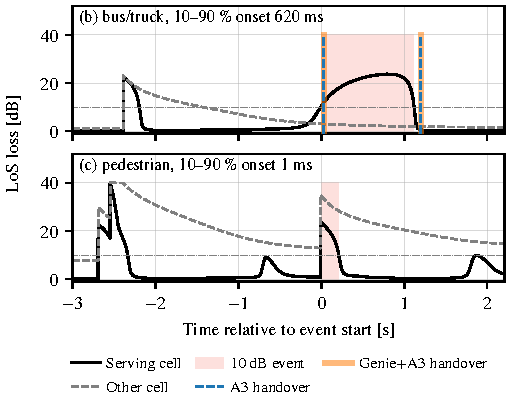
\includegraphics[width=\columnwidth]{figs/fig_onset2.pdf}
\caption{Model-B loss of (a) a typical bus/truck and (b) a typical
pedestrian outage at \SI{1}{ms} resolution, with the handover instants
of A3 and of the genie-planner at \SI{10}{dB} margin.}
\label{fig:onset}
\end{figure}

UEs experience about \numEventsPerMin{} LoS outage events (LoS loss of at
least \SI{10}{dB}) per minute, summarized by blocker class in
Table~\ref{tab:classes}. Cars never cause them. For a UE at height $h_u$
and an O-RU at height $h_o$ and horizontal distance $d$, the LoS height
at horizontal distance $x$ from the UE is $z(x)=h_u+(h_o-h_u)x/d$, which
amounts to \SI{2.7}{m}--\SI{3.3}{m} over the near lane: above a car but
through a bus or a truck (Fig.~\ref{fig:scenario}(b)). Pedestrians block
near the UE end of the link.

A blocker shadows the entire angular sector of the serving O-RU,
including the ground reflection. The strongest surviving path lies a
median of \numSameCellLoss\,dB below the unblocked LoS, so beam switching
within the same cell cannot recover the link and only a second cell can.
That cell is clear in most heavy-vehicle outages but in few pedestrian
outages, because a pedestrian close to the UE often shadows both cells.
The two classes also differ in their dynamics (Fig.~\ref{fig:onset}): the
loss caused by a bus or truck rises over \numOnsetBus\,s, whereas a
pedestrian next to the UE cuts the link almost at once, and
\numOnsetPedFast{} of pedestrian onsets last less than \SI{10}{ms}.

\subsection{Sensing Performance}
\begin{figure}[t]
\centering
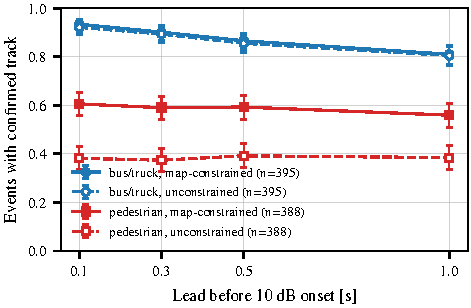
\includegraphics[width=0.9\columnwidth]{figs/fig_leadtime.pdf}
\caption{Share of outage events whose blocker is tracked a given time
before onset, for the map-constrained and the unconstrained tracker
(95\% CI).}
\label{fig:leadtime}
\end{figure}

At about \numFA{} false alarms per CPI, the track detection probability
is \numBusPd{} for buses and trucks and \numPedPd{} for pedestrians, and
a confirmed track exists \SI{0.5}{s} before onset in \numLeadBus{} of the
heavy-vehicle and \numLeadPed{} of the pedestrian outages
(Fig.~\ref{fig:leadtime}). The digital twin is used in three ways.
Static-clutter subtraction is equivalent to blind zero-Doppler removal,
because static clutter has exactly zero Doppler in simulation.
Image-method ghost rejection removes 14--21\% of the unmatched clusters
and, at a fixed false-alarm budget, raises heavy-vehicle detection from
\numGhostGain. Map-constrained tracking raises detection from \numMapBus{}
for heavy vehicles and from \numMapPed{} for pedestrians. Sensing thus
observes heavy vehicles reliably but pedestrians only about half of the
time: a pedestrian track is confirmed after a median of \numCalPedAcq\,s
and then lost for \numCalPedOut\,s at a time.

\subsection{The Value of Foresight}
\label{sec:value}
\begin{figure*}[t]
\centering
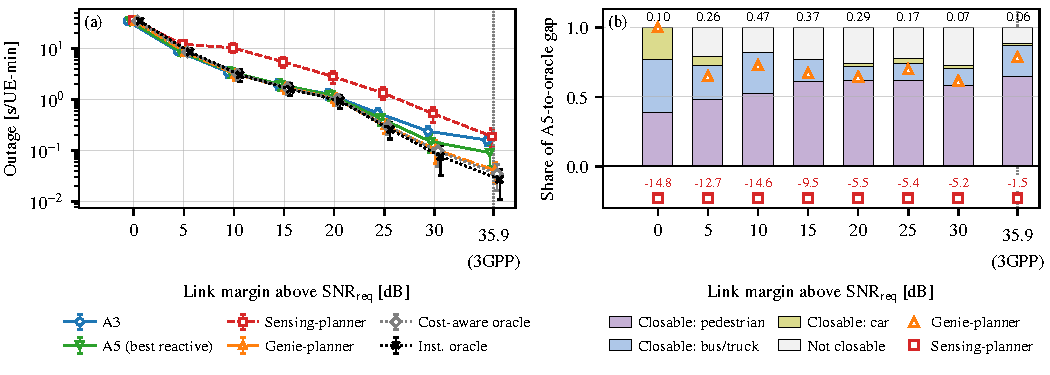
\includegraphics[width=\textwidth]{figs/fig_outage_value.pdf}
\caption{(a) Outage time at \SI{400}{Mbit/s} versus link margin for A3,
A5, the sensing-driven planner, the genie-planner
($H=\numPlanHorizon$\,s), and the two oracles (95\% CI). (b) Share of the
A5-to-oracle gap closed by the cost-aware oracle by blocker class, with
the genie-planner (triangles) and the sensing-driven planner; numbers
above the bars give the absolute gap in s/UE-min.}
\label{fig:value}
\end{figure*}

Fig.~\ref{fig:value}(a) shows the outage versus the link margin. A5, the
best reactive policy on the tuning seeds, is our reference. On the
held-out seeds it is on par with the wide-grid A3 at low margins, and its
advantage grows with the margin (\numAfiveRef{} versus
\numAthreeWideRef\,s/UE-min at the reference), because A3 hands over on
RSRP differences even when the serving cell still supports the service.

The cost-aware oracle closes \numValueRange{} of the improvable gap at
every margin from \SI{5}{dB} upward (Fig.~\ref{fig:value}(b)); at
\SI{10}{dB} it reaches \numCostOracleTen{} versus \numAfiveTen\,s/UE-min
for A5 and \numOracleTen\,s/UE-min for the instantaneous oracle. It does
so largely by making fewer, better-timed switches, and thus avoids
interruptions as well as blockage. In absolute terms, perfect foresight
lowers the outage of A5 by \numRelRedTen{} at \SI{10}{dB} and by
\numRelRedRef{} at the reference; most of the remaining outage occurs when
no cell is usable. The genie-planner closes \numGeniePlanShareRange{} of
the gap; measured against the grid-aligned oracle, which itself exceeds
the bound by at most \numGridCost, a horizon of \numPlanHorizon\,s
already suffices. Trigger
policies do not achieve this: even with perfect prediction, the trigger
genie stays at the level of the A3 it builds on (\numGenieTen{} versus
\numAthreeTen\,s/UE-min at \SI{10}{dB}), because blockage triggers ignore
sub-threshold losses and the cost of the switches they add. Foresight
therefore requires cost-aware planning but little look-ahead.

Pedestrian blockage accounts for \numValuePedRange{} of the improvable
gap and heavy vehicles for \numValueBusRange. This is the crux of the
problem: the blockers that sensing observes well cause slow outages that
A5 already follows reactively, whereas most of the value lies in abrupt
pedestrian blockage near the UE.

\subsection{Localization Requirements}
\begin{table}[t]
\centering
\caption{Error Budget: Paired Outage Difference to A5 [s/UE-min] With
Perfect Tracks and Calibrated Tracker Errors ($^\dagger$: Wilcoxon
$p\ge0.05$)}
\label{tab:errors}
\setlength{\tabcolsep}{4pt}
\begin{tabular}{@{}lcc@{}}
\toprule
Condition & \SI{10}{dB} & Reference\\
\midrule
Perfect tracks                    & \numErrPerfTen  & \numErrPerfRef\\
+ whole-track misses              & \numErrMissTen  & \numErrMissRef\\
+ persistent false tracks         & \numErrFalseTen & \numErrFalseRef\\
+ correlated pos./vel.\ error     & \numErrNoiseTen & \numErrNoiseRef\\
+ class-agnostic size rule        & \numErrSizeTen  & \numErrSizeRef\\
All tracker errors                & \numErrAllTen   & \numErrAllRef\\
All + \SI{1}{m} UE position error & \numErrAllUETen & \numErrAllUERef\\
\midrule
Real sensing-driven planner       & \numErrRealTen  & \numErrRealRef\\
\bottomrule
\end{tabular}
\end{table}

\begin{figure}[t]
\centering
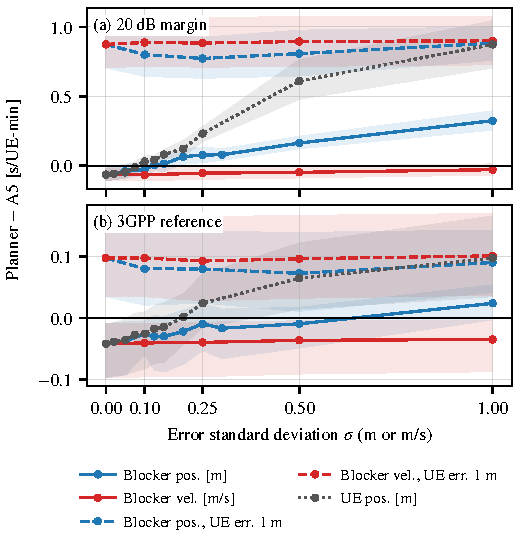
\includegraphics[width=\columnwidth]{figs/fig_error_sweep.pdf}
\caption{Accuracy requirements: outage of the planner minus that of A5
when one error source is added to perfect tracks, at \SI{20}{dB} margin
and at the reference (95\% CI). Below zero, foresight pays off.}
\label{fig:sweep}
\end{figure}

With predictions from the real tracker and a \SI{1}{m} UE position
error, the planner falls behind A5 at every margin (\numSensePlanTen{}
versus \numAfiveTen\,s/UE-min at \SI{10}{dB}), with \numSensePlanHO{}
handovers per UE-minute against \numAfiveHO{} for A5. To attribute this
shortfall, we inject the errors of our tracker into perfect tracks with
a model calibrated on the development seeds (Table~\ref{tab:errors}).
Missed tracks are the largest single cause from \SI{5}{dB} upward, and
their persistence matters: dropping detections independently per frame
costs only \numMissPerFrameTen\,s/UE-min at \SI{10}{dB}, because the
tracker bridges isolated misses. All errors together with the \SI{1}{m}
UE position error reproduce the shortfall of the real planner.

Fig.~\ref{fig:sweep} adds one error source at a time. Blocker velocity
errors up to \SI{1}{m/s} keep the outage below that of A5. For margins
of 15--\SI{30}{dB}, the break-even points lie at a blocker position error
of \numBEPosRange\,m and a UE position error of \numBEUERange\,m per
axis. With a UE position error of \SI{1}{m}, no blocker accuracy
restores the advantage. A pedestrian next to the UE is about \SI{0.5}{m}
wide, so errors of this size move it in or out of the predicted LoS; the
user's own position is the binding constraint.

\subsection{Positioning Bounds and Practical Limits}
\label{sec:posres}
\begin{figure}[t]
\centering
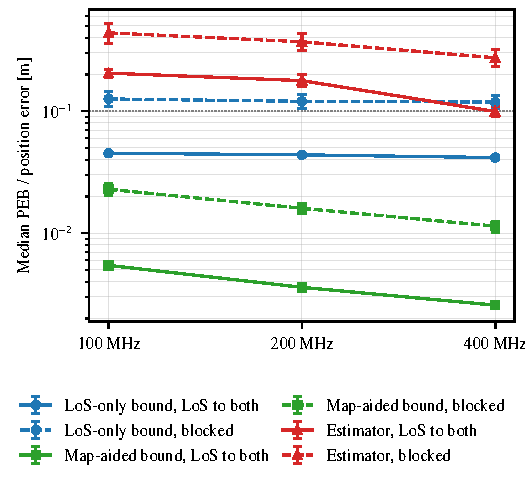
\includegraphics[width=\columnwidth]{figs/fig_p2_bw.pdf}
\caption{Median single-epoch PEB (LoS-only, map-aided) and median error of
the conference estimator \cite{natanzi2027wcncB} versus bandwidth, for
epochs with LoS to both O-RUs and with a blocked O-RU (95\% CI).}
\label{fig:bw}
\end{figure}

\begin{table*}[t]
\centering
\caption{Single-Epoch Error of the Conference Estimator
\cite{natanzi2027wcncB} at Fixed Geometries (\pValNumDraws{} Draws Each,
TDoA, no EKF) Versus the LoS-Only PEB (Biased Model); All Values in cm;
RMSE$^2$ = bias$^2$ + centered RMS$^2$}
\label{tab:val}
\setlength{\tabcolsep}{4pt}
\begin{tabular}{@{}llr|rrrr|rrrr@{}}
\toprule
 & & & \multicolumn{4}{c|}{\pBwC\,MHz} & \multicolumn{4}{c}{\pBwA\,MHz}\\
Mount & LoS state & UE $x$ [m] & PEB & bias & centered & RMSE & PEB & bias & centered & RMSE\\
\midrule
\csname @@input\endcsname tables/validation.tex
\bottomrule
\end{tabular}
\end{table*}

\textit{What limits the bound.} With LoS to both O-RUs, the LoS-only PEB
is below \pDecThr\,cm in \pDecLosFourHundredLos{} of the epochs at
\pBwC\,MHz and still in \pDecLosHundredLos{} at \pBwA\,MHz
(Fig.~\ref{fig:bw}). Relaxing one limitation at a time at \pBwB\,MHz
scales the median LoS-only PEB (\pLimLosBase\,cm) by \pLimLosBw{} for
twice the bandwidth, \pLimLosSnr{} for ten times the SNR, \pLimLosSync{}
for perfect synchronization, and \pLimLosCal{} for perfect calibration.
On these short links, the element phase errors, which bias the angles,
dominate. The map-aided PEB is much less sensitive to hardware errors
because reflections from known surfaces add independent geometric
information.

\textit{Blockage.} In the biased model, the median LoS-only PEB grows by
a factor of \pRatioLosB{} during blockage, and only
\pDecLosFourHundredBlk{} of the blocked epochs remain below \pDecThr\,cm.
If the attenuated LoS kept its geometry, the factor would be only
\pRatioLosA, which shows how optimistic it is to apply the power loss of
model~B without its geometric consequence. Map-aided information lowers
the PEB during blockage to \pMapToLosBlk{} times the LoS-only value.

\textit{Practical estimator.} The dominant-path estimator of
\cite{natanzi2027wcncB} reaches a median error of \pEstMedFourHundred\,cm
at \pBwC\,MHz (\pEstLosFourHundred\,cm with LoS to both O-RUs,
\pEstBlkFourHundred\,cm during blockage), but its 90th percentile is
\pEstPninetyFourHundred\,m. The bias--variance decomposition at fixed
geometries (Table~\ref{tab:val}) shows that the squared bias, caused by
unresolved multipath and front/back mirror solutions, dominates the
error in most geometries. Around blockage onsets the error tail grows
further: the 90th percentile rises from \pOnsetElsePninety\,m elsewhere to
\pOnsetPreHalfPninety\,m in the half second before onset, and the median
reaches \pOnsetDuringMed\,cm during the event. Fed into the planner with
perfect blocker tracks, these positions keep the outage significantly
above that of A5 at every margin, whereas synthetic errors drawn from the
map-aided bound preserve an advantage at most margins
\cite{natanzi2027wcncB}. The information to close this gap is therefore
in the signal, but the conference estimator does not extract it.

\subsection{Performance of the Proposed Tracker}
\label{sec:tracker}
\begin{figure}[t]
\centering
\placeholder{0.95\columnwidth}{4.2cm}{CDF of the position error for
unblocked and blocked epochs: conference estimator, VA tracker without
visibility prediction, proposed tracker, and samples at the map-aided
PEB.}
\caption{\textcolor{red}{[TBD]} Position error of the proposed tracker
versus the baselines, split into unblocked and blocked epochs.}
\label{fig:trackercdf}
\end{figure}

\tbd{Report median, 90th percentile, and share below \SI{10}{cm} for the
conference estimator, a VA tracker without visibility prediction
(ablation), the proposed tracker with a perfect map, and the proposed
tracker with map offsets $\sigma_{\mathrm{map}}\in\{0.1,0.25,0.5\}$\,m;
separate the windows before onset, during the event, and elsewhere as in
\cite{natanzi2027wcncB}; compare the achieved RMSE with the map-aided
PEB of Section~V-C (Fig.~\ref{fig:trackercdf}).}

\subsection{End-to-End Handover Performance}
\label{sec:e2e}
\begin{table}[t]
\centering
\caption{\textcolor{red}{[TBD]} Outage [s/UE-min], Handovers and
Ping-Pong Rate per UE-min; Held-Out Seeds, 95\% CI}
\label{tab:e2e}
\setlength{\tabcolsep}{3pt}
\begin{tabular}{@{}lcccc@{}}
\toprule
Policy & \SI{15}{dB} & Ref. & HO/min & Ping-pong\\
\midrule
A3 (tuned)                         & \newres & \newres & \newres & \newres\\
A5 (tuned)                         & \newres & \newres & \newres & \newres\\
CHO \cite{3gpp38331cho}            & \newres & \newres & \newres & \newres\\
Sensing trigger \cite{li2025lookbefore}-style & \newres & \newres & \newres & \newres\\
Learned predictor \cite{alquraan2023radar}-style & \newres & \newres & \newres & \newres\\
Planner + conf.\ estimator \cite{natanzi2027wcncB} & \newres & \newres & \newres & \newres\\
Proposed (tracker + risk-aware) & \newres & \newres & \newres & \newres\\
\quad w/o visibility prediction    & \newres & \newres & \newres & \newres\\
\quad w/o risk term ($\lambda=0$)  & \newres & \newres & \newres & \newres\\
Genie-planner                      & \newres & \newres & \newres & \newres\\
Cost-aware oracle                  & \newres & \newres & \newres & \newres\\
\bottomrule
\end{tabular}
\end{table}

\begin{figure}[t]
\centering
\placeholder{0.95\columnwidth}{4.6cm}{Outage versus link margin for all
policies of Table~\ref{tab:e2e} (95\% CI), with the cost-aware oracle as
the lower bound.}
\caption{\textcolor{red}{[TBD]} End-to-end outage versus link margin.}
\label{fig:e2e}
\end{figure}

\tbd{Present Table~\ref{tab:e2e}, Fig.~\ref{fig:e2e}, and an outage-versus-margin figure with
all policies; state the share of the value of foresight realized by the
proposed scheme; report significance against A5 and CHO; discuss which
blocker classes the gain comes from, given that pedestrians dominate the
value but are tracked only about half of the time.}

\subsection{Sensitivity, Generalization, and Complexity}
\label{sec:sens}
\begin{table}[t]
\centering
\caption{\textcolor{red}{[TBD]} Run Time per Epoch/Report}
\label{tab:complexity}
\begin{tabular}{@{}lcc@{}}
\toprule
Component & Complexity & Run time\\
\midrule
Blocker tracking & $O(N_{\mathrm{det}}N_{\mathrm{blk}})$ & \newres\\
Visibility prediction & $O(KN_{\mathrm{blk}}\sum_c|\mathcal S_c|)$ & \newres\\
Association + update & $O(I_{\mathrm{BP}}\sum_c|\mathcal S_c||\mathcal Z_c|)$ & \newres\\
Risk-aware planner & $O(K|\mathcal C|H^2/(T_r\Delta t))$ & \newres\\
\bottomrule
\end{tabular}
\end{table}

\begin{figure}[t]
\centering
\placeholder{0.95\columnwidth}{4.6cm}{Proposed scheme minus A5 versus (a)
map error $\sigma_{\mathrm{map}}$, (b) array calibration error, (c)
pedestrian density, (d) E2 delay.}
\caption{\textcolor{red}{[TBD]} Sensitivity of the end-to-end gain.}
\label{fig:sens}
\end{figure}

\tbd{Fig.~\ref{fig:sens}. Sweeps: map error $\sigma_{\mathrm{map}}$, calibration errors of the
physical array model, residual self-interference of the radar, pedestrian
and bus density, UE speed (pedestrian and vehicular UE), O-RU height,
sensing overhead, and E2 delay. Generalization: second deployment
(intersection). Validation of model~B against first-order diffraction.
Optional: validation of the pedestrian blockage predictor on DeepSense~6G
Scenario~30 \cite{alkhateeb2023deepsense}, noting the domain gap (FMCW
radar, \SI{60}{GHz} link, single base station).}

\subsection{Measured O-RAN Loop Delay}
\label{sec:e2}
\begin{figure}[t]
\centering
\placeholder{0.95\columnwidth}{3.6cm}{CDF of the measured E2 loop delay
(indication to applied control) for several report periods and numbers
of UEs, OAI rfsimulator + FlexRIC.}
\caption{\textcolor{red}{[TBD]} Measured E2 control-loop delay.}
\label{fig:e2}
\end{figure}

\tbd{Report median and 99th percentile of $\tau_{\mathrm{E2}}$
(Fig.~\ref{fig:e2}), its decomposition into transport and xApp
computation, and the effect on outage when the measured distribution
replaces the fixed \SI{20}{ms}. If the measured delay is well below the
CPI and the report period, state that the loop delay is not the
bottleneck.}

% ---------------------------------------------------------------------
\section{Discussion and Limitations}
% ---------------------------------------------------------------------
The results of Sections~\ref{sec:value} to \ref{sec:posres} explain why sensing-assisted
handover is harder than it appears. Most of the value of foresight lies in
abrupt pedestrian blockage close to the user, where both the blocker and
the user must be localized to about a decimeter, while infrastructure
radar tracks pedestrians only about half of the time and practical
positioning degrades precisely when the LoS is blocked. The proposed
tracker targets the second limitation by using the blocker tracks to
predict path visibility. \tbd{Discuss whether this suffices, and what
remains for pedestrians, e.g., UE-side or bistatic sensing that observes
the user's immediate surroundings.}

The study has limitations. It considers street-canyon deployments with
two cells \textcolor{propcol}{and one additional geometry}; monostatic
sensing at one O-RU with ideal full duplex; specular paths of limited
order without diffuse scattering; the knife-edge model~B instead of
full-wave diffraction; Shannon-based rates; and an O-RAN loop measured in
an rfsimulator rather than over the air. \tbd{update after the new
experiments.}

% ---------------------------------------------------------------------
\section{Conclusion}
% ---------------------------------------------------------------------
This paper examined ISAC-assisted proactive handover against mmWave
blockage as a complete chain from sensing through positioning to
decision in an O-RAN architecture. Against tuned service-aware reactive
handover, perfect foresight closes most of the improvable outage gap with
less than a second of look-ahead, provided that switches are planned
with their cost in mind. Harvesting this value requires the user and
nearby blockers to be localized to about a decimeter, which the
LoS-only information of the serving radio units cannot provide during
blockage, while reflected paths with known geometry can.
\tbd{Conclude with the results of the proposed tracker, the end-to-end
comparison, and the measured loop delay.}

\section*{Acknowledgment}
\tbd{Funding statement moved to the first-page footnote; add any
acknowledgments here. If AI tools were used to edit the authors' text,
disclose this here as required by the TVT instructions.}

\bibliographystyle{IEEEtran}
\bibliography{refs}

\begin{IEEEbiographynophoto}{Seyed Bagher Hashemi Natanzi}
\tbd{biography, about 100 words.}
\end{IEEEbiographynophoto}

\begin{IEEEbiographynophoto}{Bo Tang}
\tbd{biography, about 100 words.}
\end{IEEEbiographynophoto}

\end{document}
